\documentclass[article]{jlreq}
\usepackage[dvipdfmx]{graphicx}
\usepackage{here}
\usepackage{amsmath}
\usepackage{latexsym}
\usepackage{multirow}
\usepackage{textcomp}
\usepackage{url}
\usepackage{array}    % 列の設定
\usepackage{caption}
\usepackage{booktabs}
\usepackage[utf8]{inputenc}
\usepackage{subcaption}
\newcommand{\ita}{\textit}
\newcommand{\ko}{\rm{k$\Omega$}}
\newcommand{\om}{\rm$\Omega$}
\newcommand{\nf}{\rm{nF}}
\title{}
\date{}
\begin{document}\maketitle




以下に今回用いた回路を示す。ただし、$
r = 1\,\text{k}\Omega, R = 100\,\text{M}\Omega, C = 0.22\,\mu\text{F}
$
とした。
\captionsetup[subfigure]{labelformat=empty}

\begin{figure}[H]
    \centering

    \begin{subfigure}{0.45\linewidth}
        \centering
        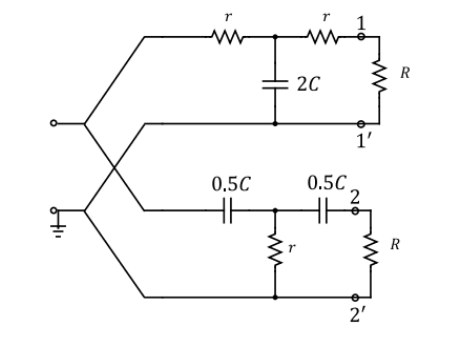
\includegraphics[width=\linewidth]{zu1.png}
        \caption{図(A)}
    \end{subfigure}
    \hfill
    \begin{subfigure}{0.53\linewidth}
        \centering
        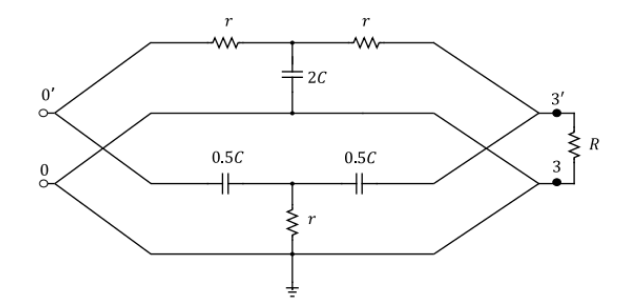
\includegraphics[width=\linewidth]{zu2.png}
        \caption{図(B)}
    \end{subfigure}
\end{figure}

\section{実験１}
\subsection{実験内容}
図(A)について、入力端子0-0'に振幅1\,Vの正弦波電圧を印加し、
周波数を$
f=100\,\mathrm{Hz}, 1\,\mathrm{kHz}, 10\,\mathrm{kHz}$
として解析を行った。

各周波数について、出力端子1-1'および2-2'の電圧波形を観測した。
また、各出力波形について理論値との比較を行った。
以下にLTspiceにより作成した各周波数に対する回路図を示す。
\setcounter{figure}{0}

\begin{figure}[H]
    \centering
    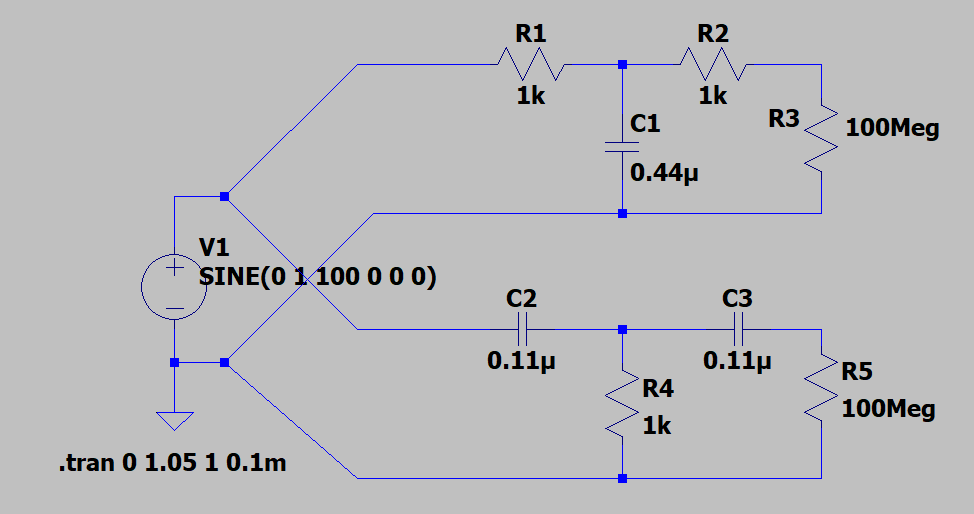
\includegraphics[scale=0.25]{kairozu2-1_100Hz.png}
    \caption{$f=100\,\mathrm{Hz}$}
\end{figure}
\begin{figure}[H]
    \centering
    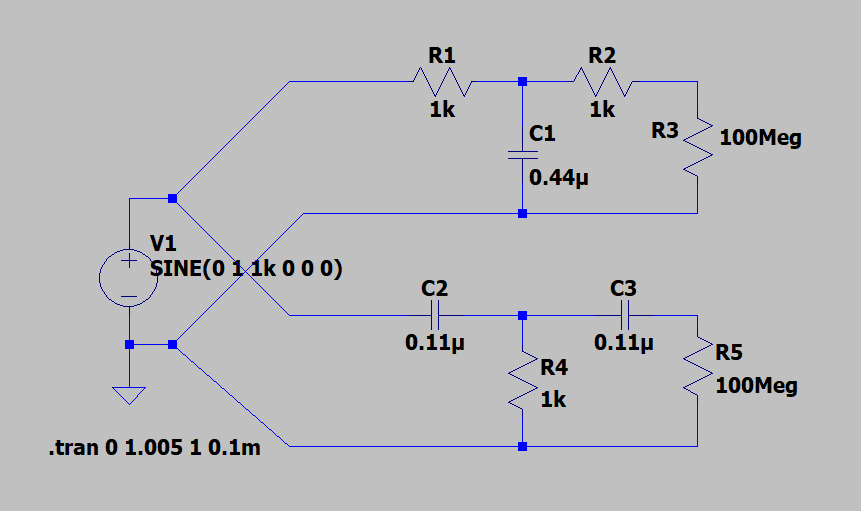
\includegraphics[scale=0.28]{kairozu2-1_1kHz.png}
    \caption{$f=1\,\mathrm{kHz}$}
\end{figure}
\begin{figure}[H]
    \centering
    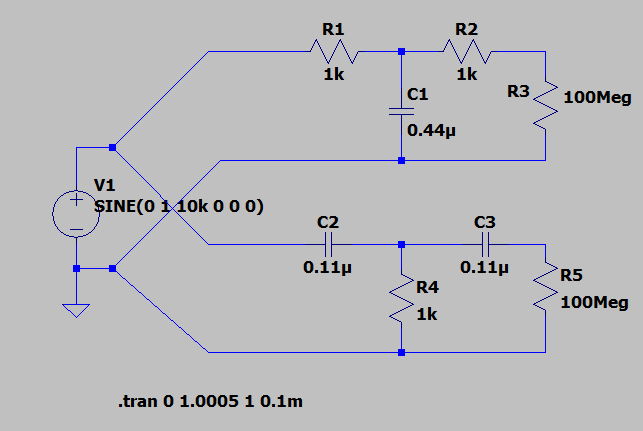
\includegraphics[scale=0.25]{kairozu2-1_10kHz.png}
    \caption{$f=10\,\mathrm{kHz}$}
\end{figure}

\subsection{結果}
各周波数に対する入出力波形を以下に示す。
ただし波形の線の色は、黄色を入力波形、青色を出力端子1-1'の波形、赤色を出力端子2-2'の波形とする。
\begin{figure}[H]
    \centering
    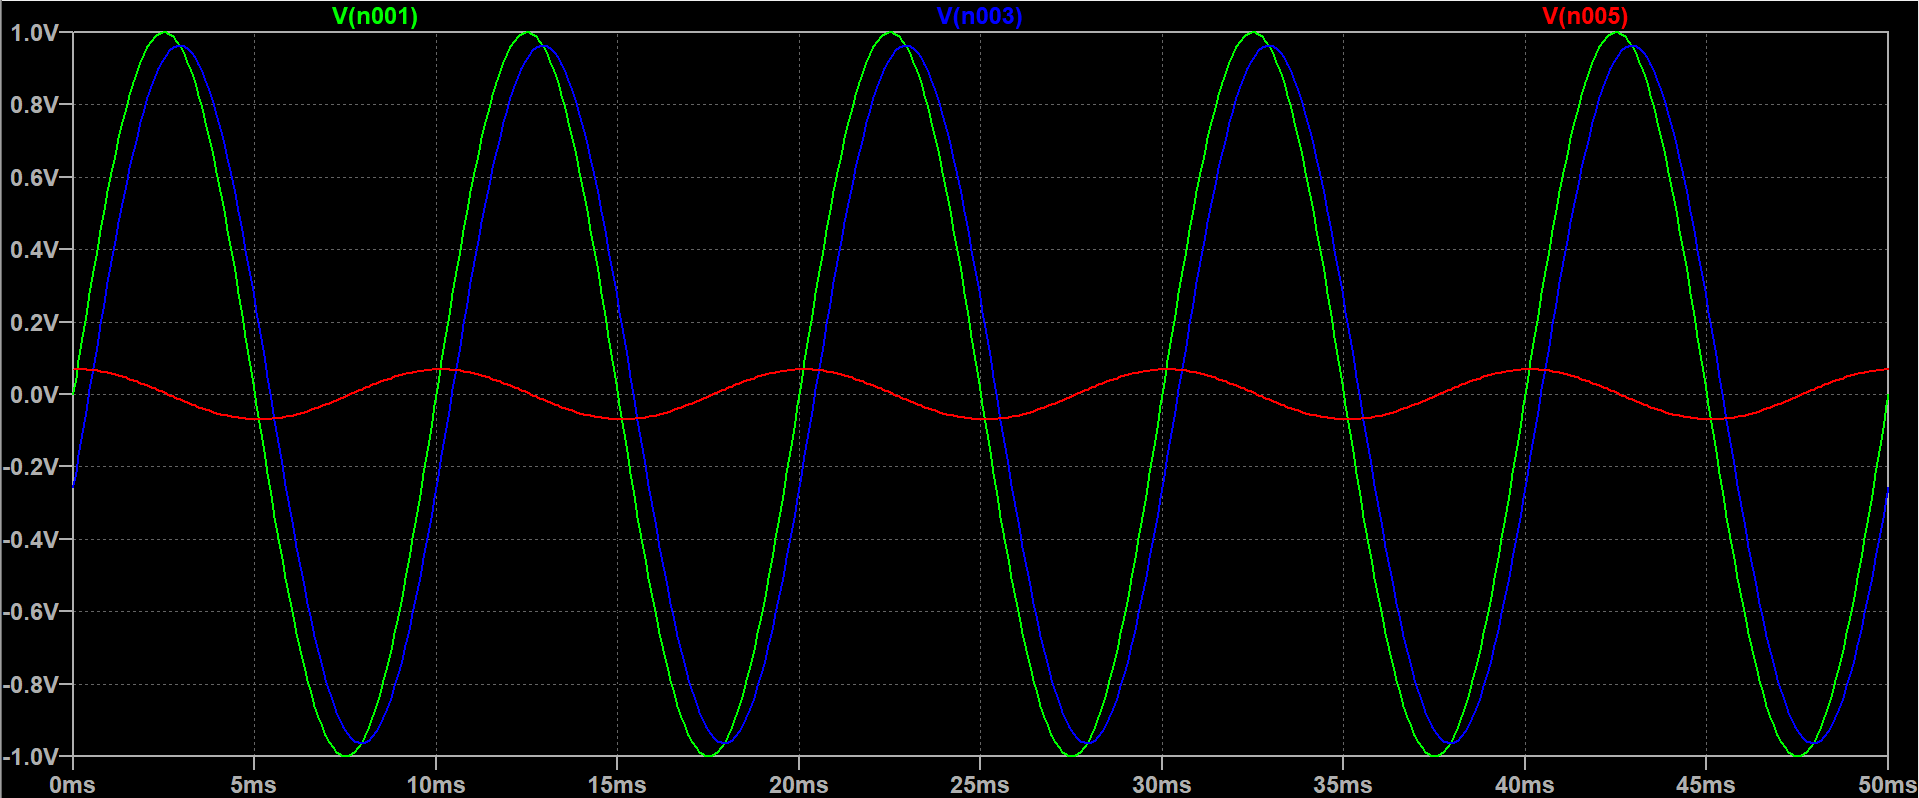
\includegraphics[scale=0.25]{sim2-1.png}
    \caption{$f=100\,\mathrm{Hz}$}
\end{figure}
\begin{figure}[H]
    \centering
    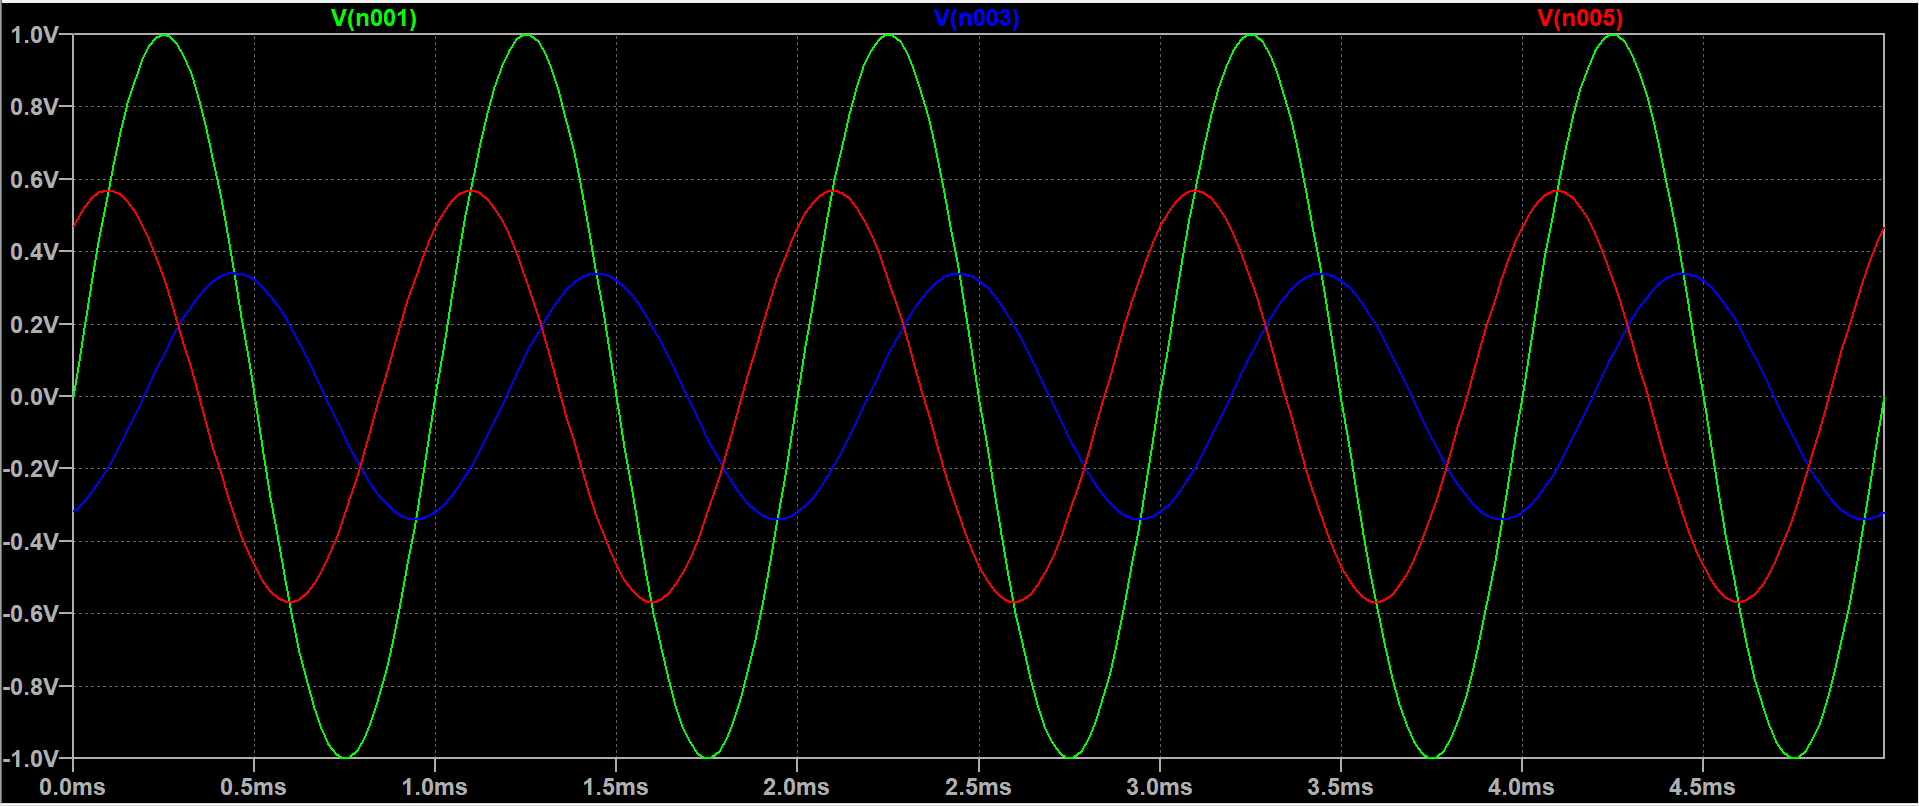
\includegraphics[scale=0.25]{sim2-2.png}
    \caption{$f=1\,\mathrm{kHz}$}
\end{figure}
\begin{figure}[H]
    \centering
    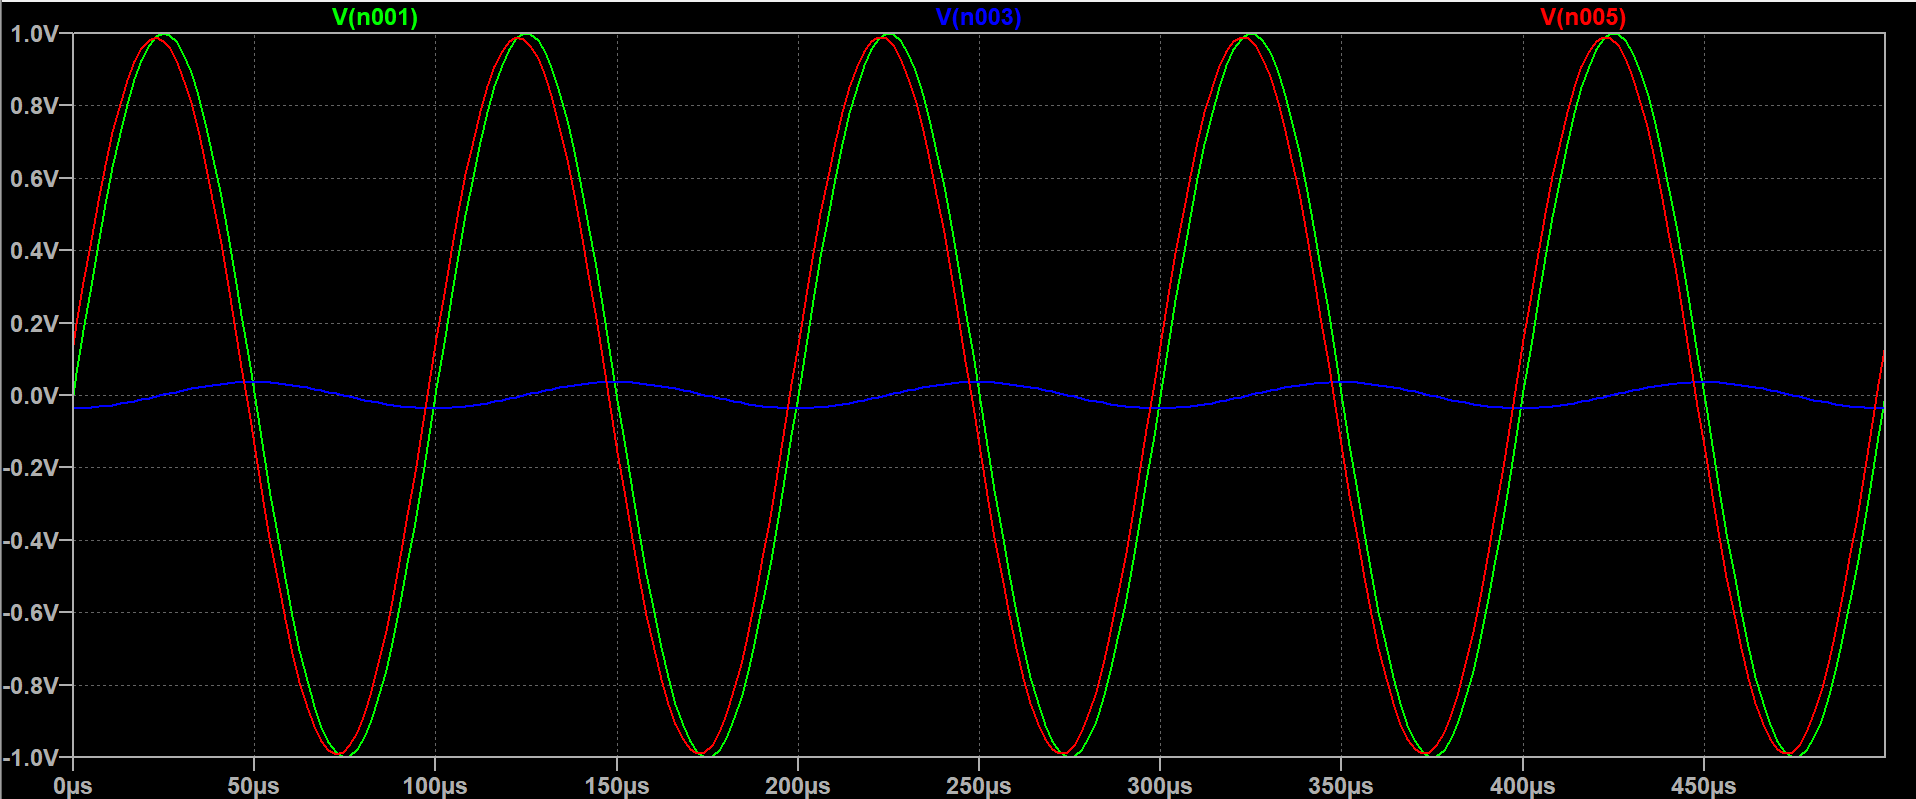
\includegraphics[scale=0.25]{sim2-3.png}
    \caption{$f=10\,\mathrm{kHz}$}
\end{figure}
\subsection{考察}
2端子対回路において、入力電圧 $V_{in}$、出力電圧 $V_{out}$、入力電流 $I_{in}$、出力電流 $I_{out}$ の関係は、インピーダンス行列 $[Z]$ を用いて次のように定義される。
\begin{equation}
\begin{bmatrix} V_{in} \\ V_{out} \end{bmatrix} = \begin{bmatrix} Z_{11} & Z_{12} \\ Z_{21} & Z_{22} \end{bmatrix} \begin{bmatrix} I_{in} \\ I_{out} \end{bmatrix}
\end{equation}
本回路において、負荷抵抗 $R$ は回路内部の抵抗 $r$ に対して十分に大きい（$R \gg r$）ため、出力端は開放（$I_{out} = 0$）とみなすことができる。このとき、伝達関数は次式で与えられる。
\begin{equation}
\frac{V_{out}}{V_{in}} = \frac{Z_{21}}{Z_{11}}
\end{equation}
図(A)における端子1-1'の出力電圧を $V_2'$、端子2-2'の出力電圧を $V_2''$ と定義する。

上部回路（端子1-1'）のインピーダンス行列 $Z'$ は、直列要素 $r$ と並列要素 $2C$ より次のように表される。
\begin{equation}
Z' = \begin{bmatrix} r + \frac{1}{j\omega 2C} & \frac{1}{j\omega 2C} \\ \frac{1}{j\omega 2C} & r + \frac{1}{j\omega 2C} \end{bmatrix}
\end{equation}
したがって、出力電圧 $V_2'$ は以下のようになる。
\begin{equation}
V_2' = \frac{\frac{1}{j\omega 2C}}{r + \frac{1}{j\omega 2C}} V_{in} = \frac{1}{1 + j\omega 2Cr} V_{in}
\end{equation}

同様に、下部回路（端子2-2'）のインピーダンス行列 $Z''$ は、直列要素 $0.5C$ と並列要素 $r$ より次のように表される。
\begin{equation}
Z'' = \begin{bmatrix} r + \frac{2}{j\omega C} & r \\ r & r + \frac{2}{j\omega C} \end{bmatrix}
\end{equation}
したがって、出力電圧 $V_2''$ は以下のようになる。
\begin{equation}
V_2'' = \frac{r}{r + \frac{2}{j\omega C}} V_{in} = \frac{j\omega Cr}{2 + j\omega Cr} V_{in}
\end{equation}

与えられた定数 $r = 1\,\text{k}\Omega$、$C = 0.22\,\mu\text{F}$ を用いると、$Cr = 2.2 \times 10^{-4}$ であり、各理論式は以下の通りとなる。
\begin{equation}
V_2' = \frac{1}{1 + j\omega (4.4 \times 10^{-4})} V_{in}
\end{equation}
\begin{equation}
V_2'' = \frac{j\omega (2.2 \times 10^{-4})}{2 + j\omega (2.2 \times 10^{-4})} V_{in}
\end{equation}

入力電圧を $V_{in}(t) = \sin(2\pi f t)$ [V] とし、各周波数における出力波形 $V_{2}(t) = A \sin(2\pi f t + \phi)$ を求める。ここで、振幅 $A$ および位相 $\phi$ は各伝達関数 $H(j\omega)$ より次のように算出される。
\begin{equation}
A = |H(j\omega)|, \quad \phi = \arg(H(j\omega))
\end{equation}

端子1-1'の伝達関数 $H_1(j\omega) = \frac{1}{1 + j\omega T_1}$ （ただし $T_1 = 4.4 \times 10^{-4}$）について、
\begin{equation}
|H_1(j\omega)| = \frac{1}{\sqrt{1 + (\omega T_1)^2}}, \quad \phi_1 = -\tan^{-1}(\omega T_1)
\end{equation}
を用いて各周波数の値を求めると、出力波形 $V_2'(t)$ は以下の通りとなる。

\begin{equation}
V_2'(t) = \begin{cases} 
0.96384 \sin(200\pi t - 0.26972) & (f = 100\,\text{Hz}) \\
0.34015 \sin(2000\pi t - 1.2237) & (f = 1\,\text{kHz}) \\
0.036148 \sin(20000\pi t - 1.5346) & (f = 10\,\text{kHz})
\end{cases}
\end{equation}

同様に、端子2-2'の伝達関数
\[
H_2(j\omega)=\frac{j\omega T_2}{2+j\omega T_2}
\]
（ただし $T_2=2.2\times10^{-4}$）について考える。

振幅は
\begin{equation}
|H_2(j\omega)|
=
\frac{\omega T_2}
{\sqrt{4+(\omega T_2)^2}}
\end{equation}
で与えられる。

また位相は複素数の偏角より
\begin{equation}
\phi_2
=
\arg(j\omega T_2)
-
\arg(2+j\omega T_2)
\end{equation}
となる。

ここで
\begin{equation}
\arg(j\omega T_2)=\frac{\pi}{2}
\end{equation}

および
\begin{equation}
\arg(2+j\omega T_2)
=
\tan^{-1}
\left(
\frac{\omega T_2}{2}
\right)
\end{equation}

より
\begin{equation}
\phi_2
=
\frac{\pi}{2}
-
\tan^{-1}
\left(
\frac{\omega T_2}{2}
\right)
\end{equation}

となる。

以上を用いて算出すると，出力波形
$V_2''(t)$ は以下の通りとなる。

\begin{equation}
V_2''(t) = \begin{cases} 
0.068867 \sin(200\pi t + 1.5019) & (f = 100\,\text{Hz}) \\
0.56788 \sin(2000\pi t + 0.96668) & (f = 1\,\text{kHz}) \\
0.98982 \sin(20000\pi t + 0.14418) & (f = 10\,\text{kHz})
\end{cases}
\end{equation}


式(11)と式(17)に$t$を代入した理論値と測定値をまとめた表を以下に示す。

\begin{table}[H]
\centering
\caption{端子1-1'における理論値と測定値（100 Hz）}
\begin{tabular}{cccc}
\toprule
$t$ [s] & 理論値 [V] & 測定値 [V] & 相対誤差 \\
\midrule
0     & -0.25683 & -0.25689 & $2.34\times10^{-4}$ \\
0.001 & 0.33827  & 0.33802  & $7.39\times10^{-4}$ \\
0.002 & 0.80416  & 0.80369  & $5.84\times10^{-4}$ \\
0.003 & 0.96289  & 0.96238  & $5.30\times10^{-4}$ \\
0.004 & 0.75383  & 0.75348  & $4.64\times10^{-4}$ \\
0.005 & 0.25683  & 0.25677  & $2.34\times10^{-4}$ \\
0.006 & -0.33827 & -0.33801 & $7.69\times10^{-4}$ \\
0.007 & -0.80416 & -0.80369 & $5.84\times10^{-4}$ \\
0.008 & -0.96289 & -0.96238 & $5.30\times10^{-4}$ \\
0.009 & -0.75383 & -0.75348 & $4.64\times10^{-4}$ \\
0.010 & -0.25683 & -0.25677 & $2.34\times10^{-4}$ \\
\bottomrule
\end{tabular}
\end{table}
\begin{table}[H]
\centering
\caption{端子2-2'における理論値と測定値（100 Hz）}
\begin{tabular}{cccc}
\toprule
$t$ [s] & 理論値 [V] & 測定値 [V] & 相対誤差 \\
\midrule
0     & 0.068786 & 0.068808 & $3.20\times10^{-4}$ \\
0.001 & 0.058444 & 0.058429 & $2.57\times10^{-4}$ \\
0.002 & 0.025778 & 0.025765 & $5.04\times10^{-4}$ \\
0.003 & -0.01673 & -0.01674 & $5.98\times10^{-4}$ \\
0.004 & -0.05285 & -0.05285 & $0$ \\
0.005 & -0.06879 & -0.06877 & $2.91\times10^{-4}$ \\
0.006 & -0.05844 & -0.05843 & $1.71\times10^{-4}$ \\
0.007 & -0.02578 & -0.02577 & $3.88\times10^{-4}$ \\
0.008 & 0.016735 & 0.016740 & $2.99\times10^{-4}$ \\
0.009 & 0.052855 & 0.052851 & $7.57\times10^{-5}$ \\
0.010 & 0.068786 & 0.068775 & $1.60\times10^{-4}$ \\
\bottomrule
\end{tabular}
\end{table}

\begin{table}[H]
\centering
\caption{端子1-1'における理論値と測定値（1 kHz）}
\begin{tabular}{cccc}
\toprule
$t$ [s] & 理論値 [V] & 測定値 [V] & 相対誤差 \\
\midrule
0      & -0.31987 & -0.31679 & $9.62\times10^{-3}$ \\
0.0001 & -0.19077 & -0.18760 & $1.66\times10^{-2}$ \\
0.0002 & 0.011194 & 0.013161 & $1.76\times10^{-1}$ \\
0.0003 & 0.20888  & 0.20995  & $5.10\times10^{-3}$ \\
0.0004 & 0.32678  & 0.32725  & $1.44\times10^{-3}$ \\
0.0005 & 0.31987  & 0.32015  & $9.06\times10^{-4}$ \\
0.0006 & 0.19077  & 0.19124  & $2.49\times10^{-3}$ \\
0.0007 & -0.011194 & -0.010339 & $7.61\times10^{-2}$ \\
0.0008 & -0.20888 & -0.20777 & $5.32\times10^{-3}$ \\
0.0009 & -0.32678 & -0.32559 & $3.65\times10^{-3}$ \\
0.0010 & -0.31987 & -0.31885 & $3.18\times10^{-3}$ \\
\bottomrule
\end{tabular}
\end{table}

\begin{table}[H]
\centering
\caption{端子2-2'における理論値と測定値（1 kHz）}
\begin{tabular}{cccc}
\toprule
$t$ [s] & 理論値 [V] & 測定値 [V] & 相対誤差 \\
\midrule
0      & 0.46772  & 0.47056  & $6.07\times10^{-3}$ \\
0.0001 & 0.56841  & 0.56848  & $1.31\times10^{-4}$ \\
0.0002 & 0.45198  & 0.45197  & $2.47\times10^{-5}$ \\
0.0003 & 0.16291  & 0.16322  & $1.88\times10^{-3}$ \\
0.0004 & -0.18838 & -0.18793 & $2.38\times10^{-3}$ \\
0.0005 & -0.46772 & -0.46725 & $1.01\times10^{-3}$ \\
0.0006 & -0.56841 & -0.56807 & $5.97\times10^{-4}$ \\
0.0007 & -0.45198 & -0.45190 & $1.69\times10^{-4}$ \\
0.0008 & -0.16291 & -0.16318 & $1.69\times10^{-3}$ \\
0.0009 & 0.18839  & 0.18805  & $1.76\times10^{-3}$ \\
0.0010 & 0.46772  & 0.46747  & $5.50\times10^{-4}$ \\
\bottomrule
\end{tabular}
\end{table}

\begin{table}[H]
\centering
\caption{端子1-1'における理論値と測定値（10 kHz）}
\begin{tabular}{cccc}
\toprule
$t$ [s] & 理論値 [V] & 測定値 [V] & 相対誤差 \\
\midrule
0        & -0.036124 & -0.035482 & $1.77\times10^{-2}$ \\
0.00001  & -0.028457 & -0.027720 & $2.60\times10^{-2}$ \\
0.00002  & -0.0099203 & -0.0092586 & $6.67\times10^{-2}$ \\
0.00003  & 0.012406 & 0.012990 & $4.71\times10^{-2}$ \\
0.00004  & 0.029993 & 0.030516 & $1.74\times10^{-2}$ \\
0.00005  & 0.036124 & 0.036618 & $1.37\times10^{-2}$ \\
0.00006  & 0.028457 & 0.028958 & $1.76\times10^{-2}$ \\
0.00007  & 0.0099203 & 0.010459 & $5.43\times10^{-2}$ \\
0.00008  & -0.012406 & -0.011825 & $4.68\times10^{-2}$ \\
0.00009  & -0.029993 & -0.029385 & $2.03\times10^{-2}$ \\
0.00010  & -0.036124 & -0.035514 & $1.68\times10^{-2}$ \\
\bottomrule
\end{tabular}
\end{table}

\begin{table}[H]
\centering
\caption{端子2-2'における理論値と測定値（10 kHz）}
\begin{tabular}{cccc}
\toprule
$t$ [s] & 理論値 [V] & 測定値 [V] & 相対誤差 \\
\midrule
0        & 0.14172  & 0.13927  & $1.73\times10^{-2}$ \\
0.00001  & 0.69039  & 0.68664  & $5.43\times10^{-3}$ \\
0.00002  & 0.97535  & 0.97135  & $4.10\times10^{-3}$ \\
0.00003  & 0.88776  & 0.88470  & $3.45\times10^{-3}$ \\
0.00004  & 0.46108  & 0.45883  & $4.88\times10^{-3}$ \\
0.00005  & -0.14172 & -0.14299 & $8.95\times10^{-3}$ \\
0.00006  & -0.69039 & -0.69082 & $6.18\times10^{-4}$ \\
0.00007  & -0.97535 & -0.97535 & $5.64\times10^{-7}$ \\
0.00008  & -0.88776 & -0.88819 & $4.86\times10^{-4}$ \\
0.00009  & -0.46108 & -0.46188 & $1.74\times10^{-3}$ \\
0.00010  & 0.14172  & 0.14041  & $9.22\times10^{-3}$ \\
\bottomrule
\end{tabular}
\end{table}

図(A)における各周波数の出力波形について、理論値とシミュレーション結果を比較する。

まず、1-1'端子の出力について考える。伝達関数は
\[
H_1(j\omega)=\frac{1}{1+j\omega 2Cr}
\]
で与えられる。この式より、$\omega$が大きくなると分母の$j\omega 2Cr$の影響が大きくなり、$|H_1(j\omega)|$は小さくなる。実際に、周波数を100\,Hzから10\,kHzへと増加させると、出力振幅が減少していることが確認できる。

次に、2-2'端子の出力について考える。伝達関数は
\[
H_2(j\omega)=\frac{j\omega Cr}{2+j\omega Cr}
\]
である。この式より、$\omega$が小さいときは分子が小さくなり出力は小さいが，$\omega$が大きくなると分母の$j\omega Cr$が支配的となり，$|H_2(j\omega)|$は1に近づく。実際に、周波数の増加に伴い出力振幅が大きくなることが確認された。

また、理論値と測定値を比較すると、いずれの周波数においても波形はよく一致しており，相対誤差は最大でも$10^{-2}$程度であった。特に100\,Hzおよび1\,kHzでは誤差は$10^{-3}$程度と小さく，理論解析が妥当であることが確認できる。

一方で、10\,kHzにおいては1-1'端子の出力振幅が非常に小さいため、相対誤差がやや大きくなる傾向が見られた。これは絶対誤差自体は小さいものの、理論値が小さいことによるものである。

さらに、シミュレーションにおいては1周期後の値が完全には一致せず、
わずかな差が生じている。
この原因について過渡現象の影響を考察した。

まず100\,Hzの場合について考える。1-1'端子の時定数は
\[
\tau_1=2Cr=4.4\times10^{-4}\,\mathrm{s}
\]
であり、
\[
5\tau_1=2.2\times10^{-3}\,\mathrm{s}
\]
となる。また2-2'端子の時定数は
\[
\tau_2=\frac{Cr}{2}=1.1\times10^{-4}\,\mathrm{s}
\]
であり、
\[
5\tau_2=5.5\times10^{-4}\,\mathrm{s}
\]
となる。一方、100\,Hzの周期は
\[
T=\frac{1}{100}=1.0\times10^{-2}\,\mathrm{s}
\]
であり、
\[
T \gg 5\tau_1,\ 5\tau_2
\]
が成り立つ。したがって、1周期後には過渡成分は十分に減衰していると考えられる。
よって、100\,Hzにおける差はLTspiceの数値計算における丸め誤差などによるものと考えられる。

次に1\,kHzの場合について考える。周期は
\[
T=1.0\times10^{-3}\,\mathrm{s}
\]
であり、
\[
T < 5\tau_1=2.2\times10^{-3}\,\mathrm{s}
\]
かつ
\[
T > 5\tau_2=5.5\times10^{-4}\,\mathrm{s}
\]
である。このため、1周期後の時点では特に1-1'端子において
過渡成分が完全には消滅していない可能性があると考えられる。

また10\,kHzの場合については、周期は
\[
T=1.0\times10^{-4}\,\mathrm{s}
\]
であり、
\[
T < 5\tau_1,\ 5\tau_2
\]
が成り立つ。したがって、両端子において1周期後には
過渡成分が残っている可能性があると考えられる。

そこで、1周期目以降の値についても解析を行った。
以下にその結果を示す。
\begin{table}[H]
\centering
\caption{1 kHzにおける各周期の同一位相での出力電圧}
\begin{tabular}{ccc}
\toprule
時刻 $t$ [s] & $V'$ [V] & $V''$ [V] \\
\midrule
0      & -0.31679 & 0.47056 \\
0.001  & -0.31885 & 0.46747 \\
0.002  & -0.31925 & 0.46759 \\
0.003  & -0.31930 & 0.46761 \\
0.004  & -0.31930 & 0.46761 \\
\bottomrule
\end{tabular}
\end{table}

\begin{table}[H]
\centering
\caption{10 kHzにおける各周期の同一位相での出力電圧}
\begin{tabular}{ccc}
\toprule
時刻 $t$ [s]  & $V'$ [V] & $V''$ [V] \\
\midrule
0        & -0.035482 & 0.13927 \\
0.0001   & -0.035514 & 0.14041 \\
0.0002   & -0.035629 & 0.14105 \\
0.0003   & -0.035716 & 0.14130 \\
0.0004   & -0.035784 & 0.14140 \\
\bottomrule
\end{tabular}
\end{table}

これらの表より、
1\,kHzでは $t=0.002\,\mathrm{s}$ 以降、
10\,kHzでは $t=0.0003\,\mathrm{s}$ 以降の値がほぼ一定となっており、
時間の経過とともに定常状態に近づいていることが確認できた。

以上より、1\,kHzおよび10\,kHzにおける1周期後の値の差は、
LTspiceの数値計算による誤差に加えて、
過渡成分の影響もわずかに含まれていると考えられる。

\section{実験2}
\subsection{実験内容}
図(B)について、実験1と同じ条件で
入力端子0-0'に正弦波電圧を印加し、周波数$
f=100\,\mathrm{Hz}, 1\,\mathrm{kHz}, 10\,\mathrm{kHz}$に対する
出力端子3-3'の応答波形を観測した。以下にLTspiceにより作成した各周波数に対する回路図を示す。

\begin{figure}[H]
    \centering
    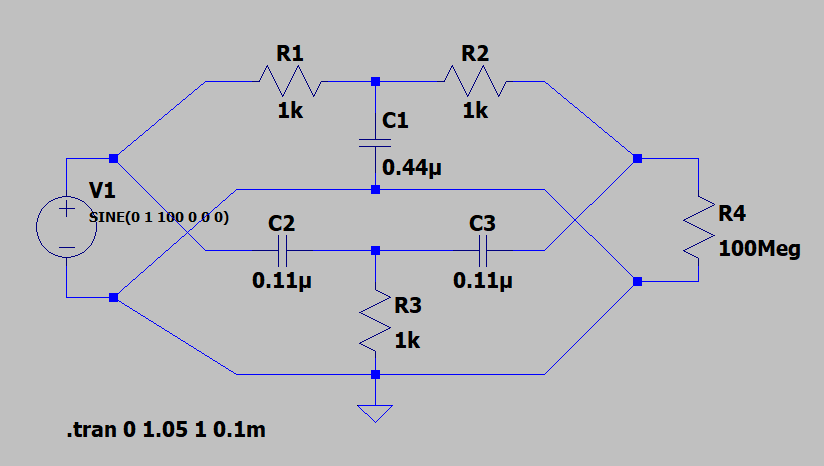
\includegraphics[scale=0.25]{kairozu2-2_100Hz.png}
    \caption{$f=100\,\mathrm{Hz}$}
\end{figure}
\begin{figure}[H]
    \centering
    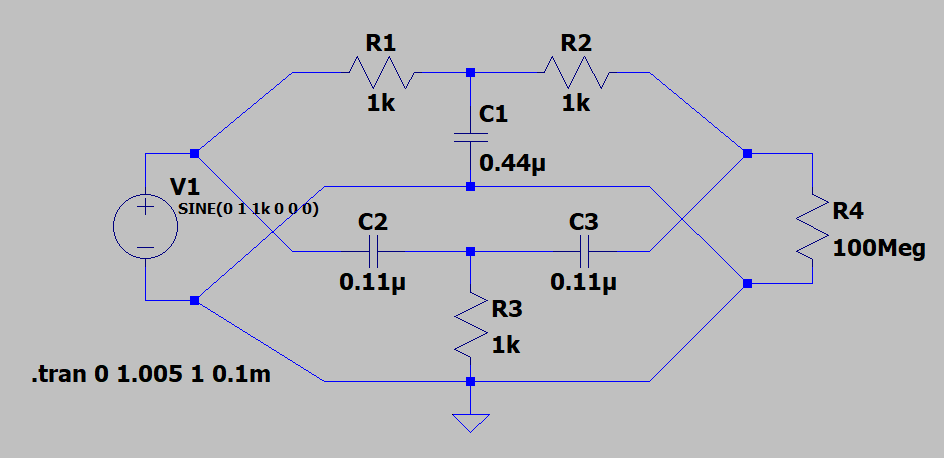
\includegraphics[scale=0.25]{kairozu2-2_1kHz.png}
    \caption{$f=1\,\mathrm{kHz}$}
\end{figure}
\begin{figure}[H]
    \centering
    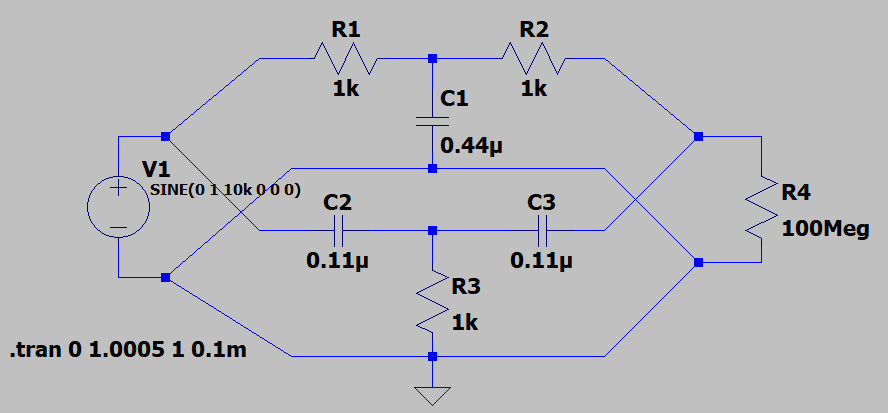
\includegraphics[scale=0.25]{kairozu2-2_10kHz.png}
    \caption{$f=10\,\mathrm{kHz}$}
\end{figure}
\subsection{結果}

各周波数に対する入出力波形を以下に示す。
ただし、青色を入力波形、黄色を出力端子3-3'の波形とする。
\begin{figure}[H]
    \centering
    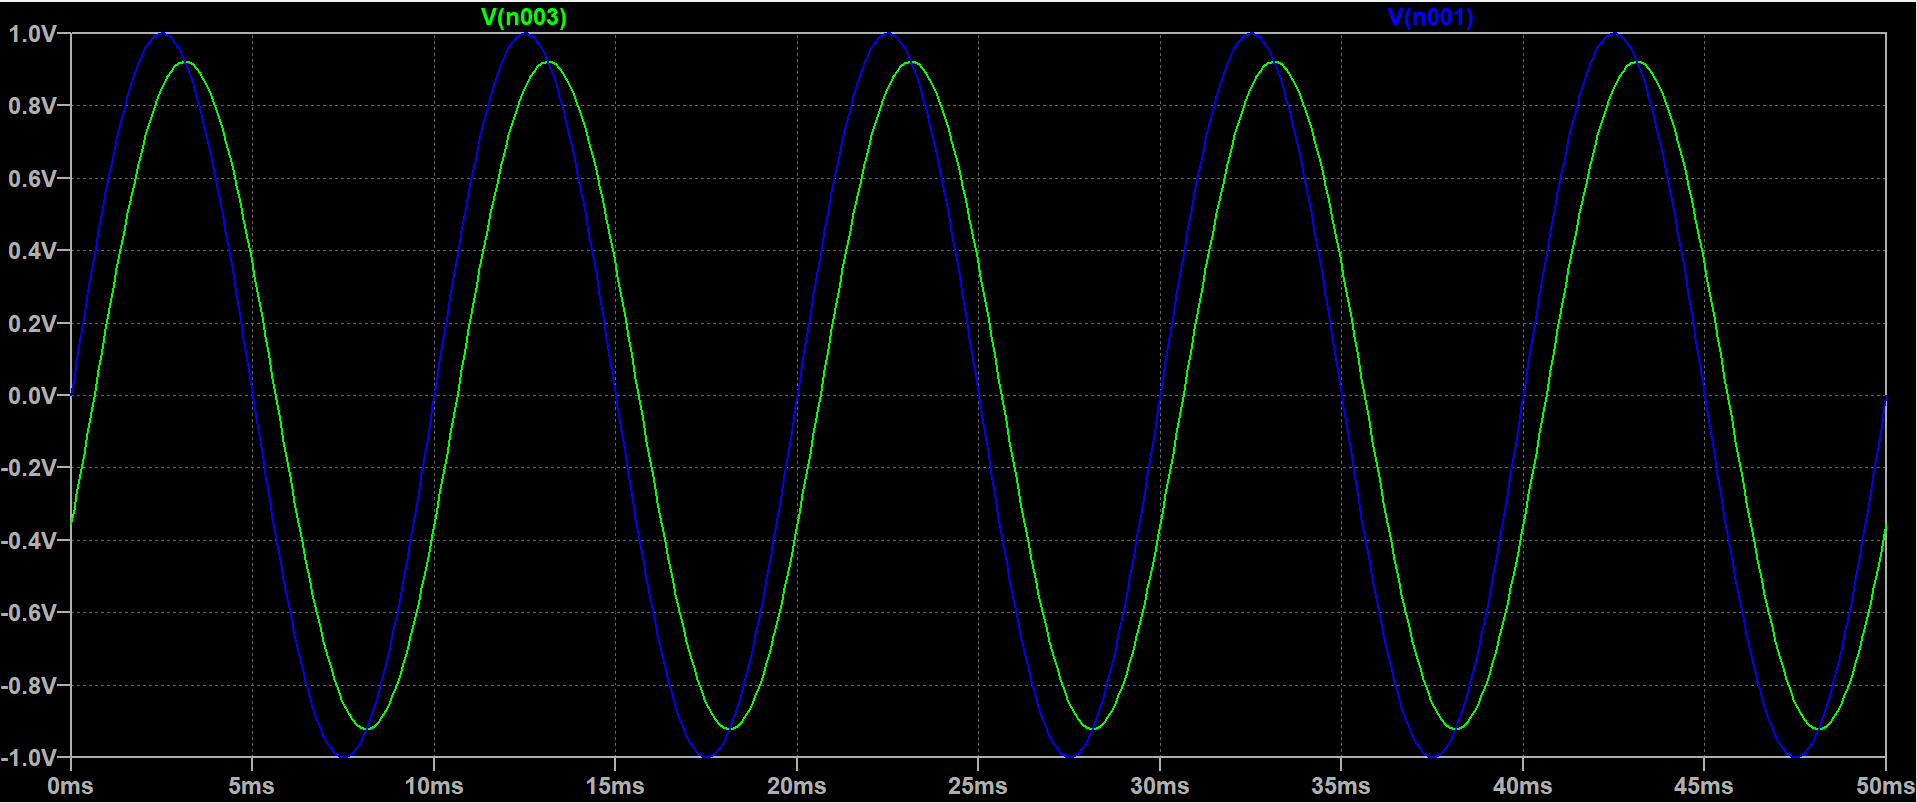
\includegraphics[scale=0.25]{sim2-4.png}
    \caption{$f=100\,\mathrm{Hz}$}
\end{figure}
\begin{figure}[H]
    \centering
    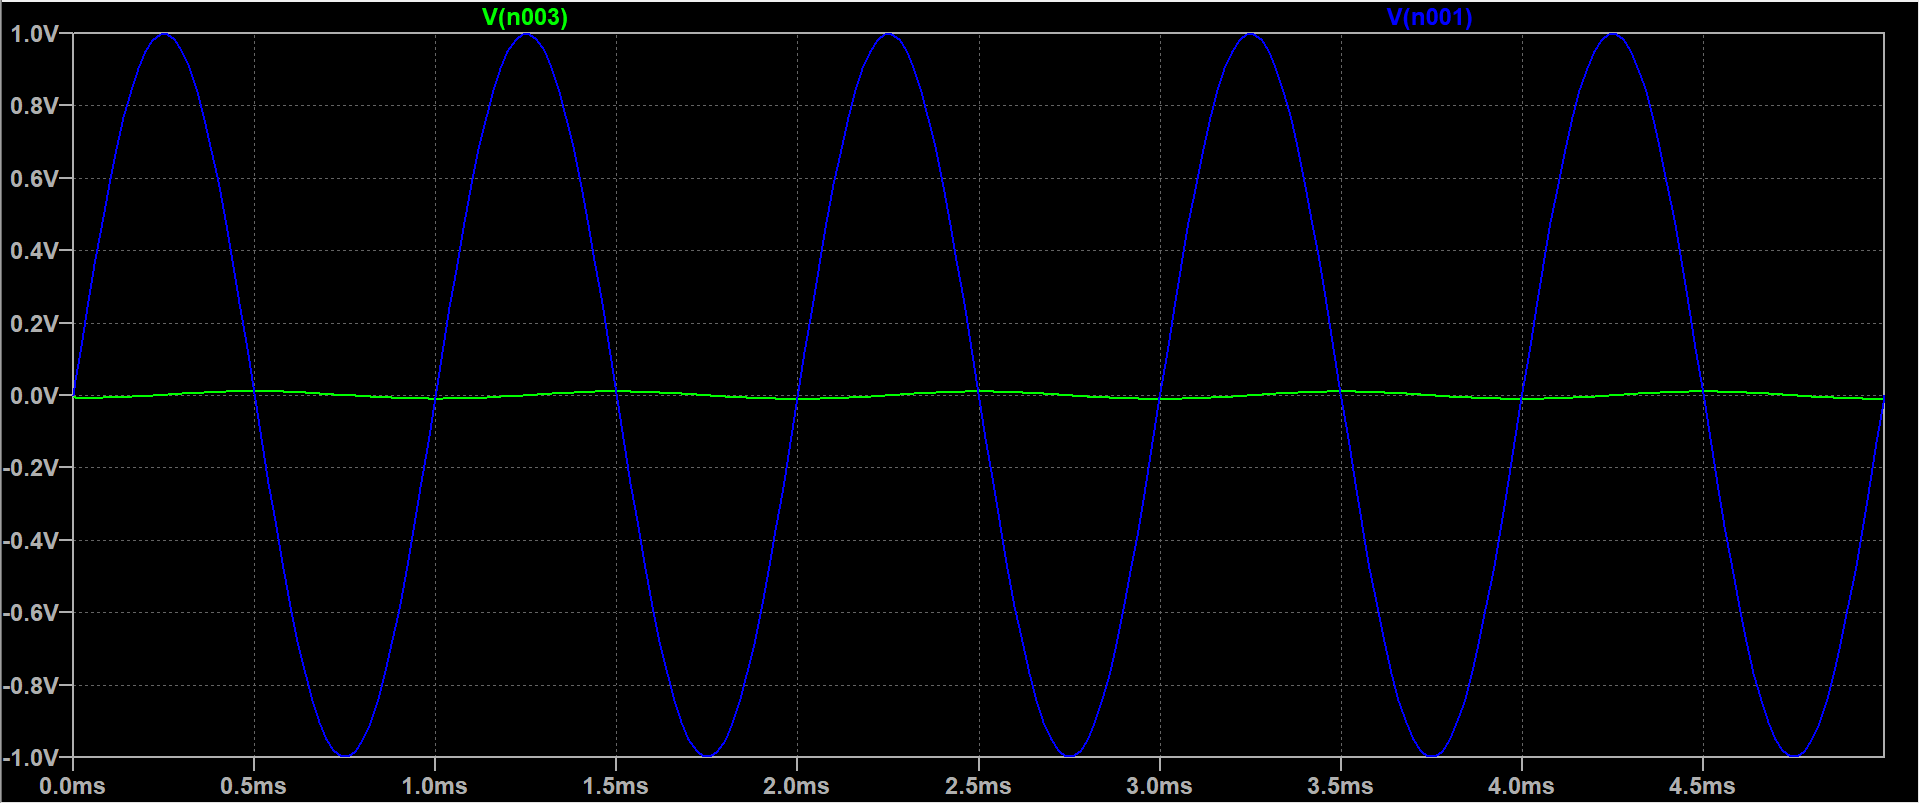
\includegraphics[scale=0.25]{sim2-5.png}
    \caption{$f=1\,\mathrm{kHz}$}
\end{figure}
\begin{figure}[H]
    \centering
    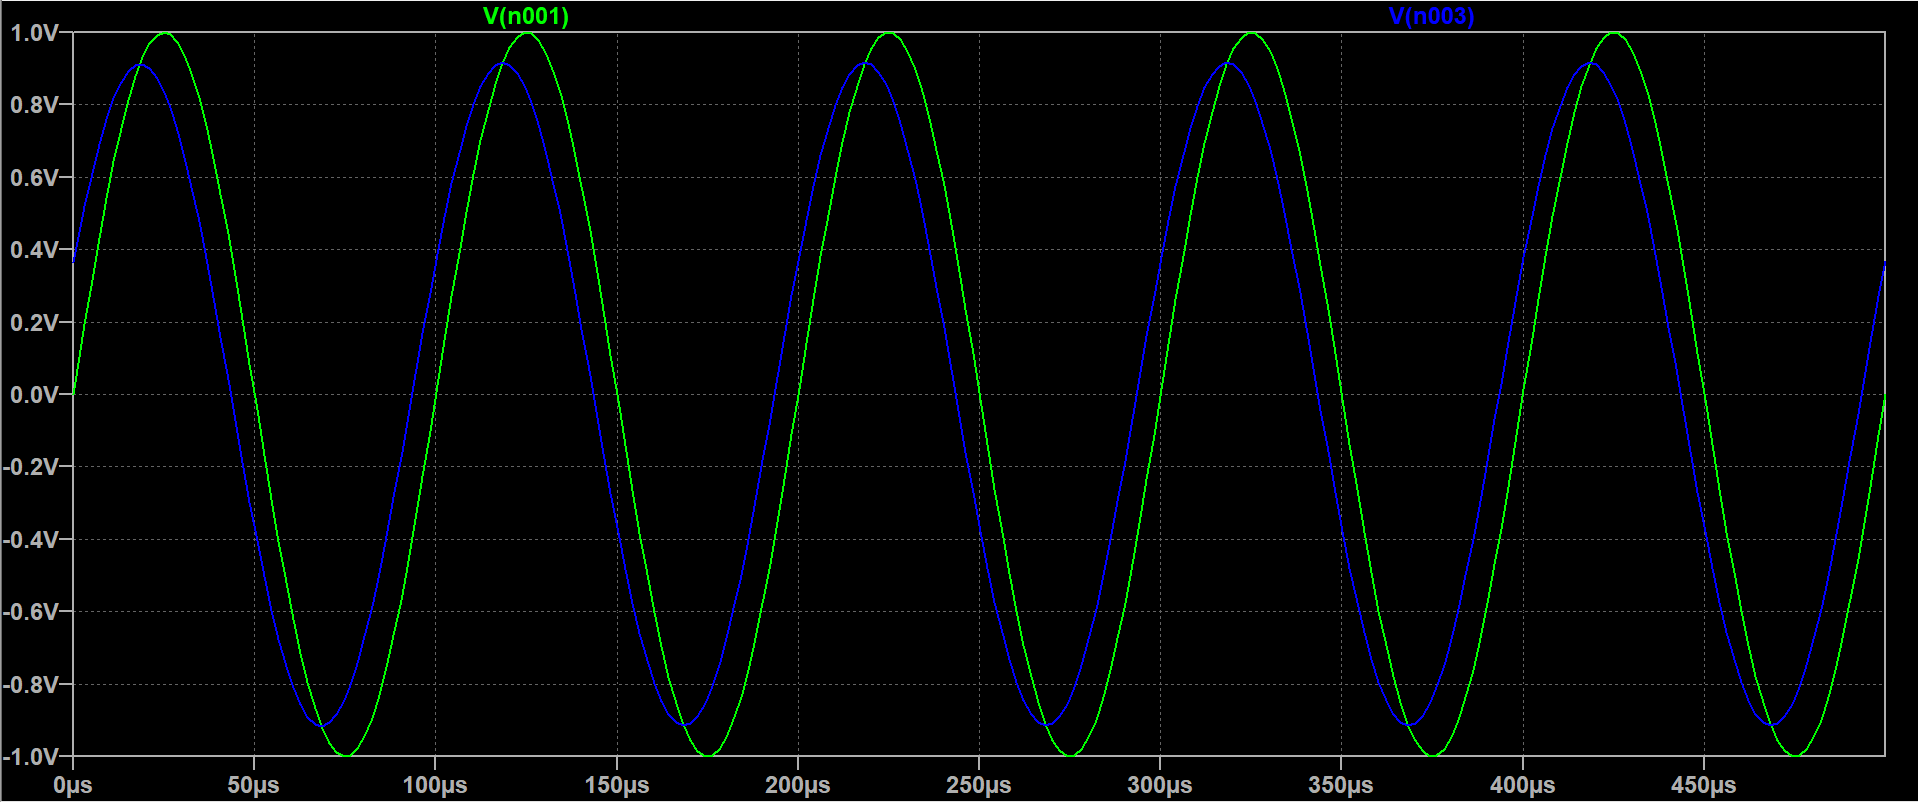
\includegraphics[scale=0.25]{sim2-6.png}
    \caption{$f=10\,\mathrm{kHz}$}
\end{figure}
\subsection{考察}
図(B)は2つのT型2端子対回路の並列接続とみなせる。
抵抗2個を含む回路のアドミタンス行列を $Y_1$、
キャパシタ2個を含む回路のアドミタンス行列を $Y_2$ とすると，

\begin{equation}
Y=Y_1+Y_2
\end{equation}

である。

入力電流 $I_0$，出力電流 $I_3$、
入力電圧 $V_0$，出力電圧 $V_3$ は

\begin{equation}
\begin{bmatrix}
I_0 \\
I_3
\end{bmatrix}
=
\begin{bmatrix}
Y_{11} & Y_{12} \\
Y_{21} & Y_{22}
\end{bmatrix}
\begin{bmatrix}
V_0 \\
V_3
\end{bmatrix}
\end{equation}

と表される。

出力端は開放とみなし

\begin{equation}
I_3=0
\end{equation}

とすると，

\begin{equation}
0=Y_{21}V_0+Y_{22}V_3
\end{equation}

より

\begin{equation}
V_3
=
-\frac{Y_{21}}{Y_{22}}V_0
\end{equation}

したがって伝達関数は

\begin{equation}
H_B(j\omega)
=
\frac{V_3}{V_0}
=
-\frac{Y_{21}}{Y_{22}}
\end{equation}

となる。

各部分回路のアドミタンス行列は

\begin{equation}
Y_1=
\frac{1}{
r\left(
r+\frac1{j\omega C}
\right)
}
\begin{bmatrix}
r+\frac1{2j\omega C}
&
-\frac1{2j\omega C}
\\
-\frac1{2j\omega C}
&
r+\frac1{2j\omega C}
\end{bmatrix}
\end{equation}

\begin{equation}
Y_2=
\frac1{
\frac2{j\omega C}
\left(
\frac2{j\omega C}+2r
\right)
}
\begin{bmatrix}
r+\frac2{j\omega C}
&
-r
\\
-r
&
r+\frac2{j\omega C}
\end{bmatrix}
\end{equation}

したがって

\begin{equation}
Y_{21}
=
-\left(
\frac{
\frac1{2j\omega C}
}{
r\left(
r+\frac1{j\omega C}
\right)
}
+
\frac{
r
}{
\frac2{j\omega C}
\left(
\frac2{j\omega C}+2r
\right)
}
\right)
\end{equation}

\begin{equation}
Y_{22}
=
\frac{
r+\frac1{2j\omega C}
}{
r\left(
r+\frac1{j\omega C}
\right)
}
+
\frac{
r+\frac2{j\omega C}
}{
\frac2{j\omega C}
\left(
\frac2{j\omega C}+2r
\right)
}
\end{equation}

これらを代入すると

\begin{equation}
H_B(j\omega)
=
\frac{
\frac1{2j\omega C}
\cdot
\frac2{j\omega C}
\left(
\frac2{j\omega C}+2r
\right)
+
r^2
\left(
r+\frac1{j\omega C}
\right)
}{
\frac2{j\omega C}
\left(
\frac2{j\omega C}+2r
\right)
\left(
r+\frac1{2j\omega C}
\right)
+
r
\left(
r+\frac1{j\omega C}
\right)
\left(
r+\frac2{j\omega C}
\right)
}
\end{equation}

ここで


\begin{equation}
m=\omega Cr
\end{equation}

とおくと

\begin{equation}
H_B(j\omega)
=
\frac{
(m^6-3m^4+4)
+j6(m^5-m^3-2m)
}{
m^6+33m^4+36m^2+4
}
\end{equation}

そして、$r = 1\,\text{k}\Omega$、$C = 0.22\,\mu\text{F}$ を使い各周波数について，振幅

\begin{equation}
A=|H_B(j\omega)|
\end{equation}

および位相差

\begin{equation}
\phi=
\tan^{-1}
\left(
\frac{
6(m^5-m^3-2m)
}{
m^6-3m^4+4
}
\right)
\end{equation}

を求めると、端子3-3'における出力波形は次のようになる。

\begin{equation}
V_B=
\begin{cases}
0.92241\sin(200\pi t-0.39651)
&(f = 100\,\text{Hz})
\\
0.010760\sin(2000\pi t-1.56004)
&(f = 1\,\mathrm{kHz})
\\
0.91577\sin(20000\pi t+0.41338)
&(f = 10\,\mathrm{kHz})
\end{cases}
\end{equation}

この式に$t$を代入したときの理論値と測定値をまとめた表を以下に示す。


\begin{table}[H]
\centering
\caption{端子3-3'における理論値と測定値（100 Hz）}
\begin{tabular}{cccc}
\toprule
$t$ [s] & 理論値 [V] & 測定値 [V] & 相対誤差 \\
\midrule
0     & -0.35624 & -0.35631 & $1.96\times10^{-4}$ \\
0.001 & 0.21191  & 0.21169  & $1.04\times10^{-3}$ \\
0.002 & 0.69912  & 0.69866  & $6.58\times10^{-4}$ \\
0.003 & 0.91929  & 0.91876  & $5.77\times10^{-4}$ \\
0.004 & 0.78832  & 0.78793  & $4.95\times10^{-4}$ \\
0.005 & 0.35624  & 0.35614  & $2.81\times10^{-4}$ \\
0.006 & -0.21191 & -0.21169 & $1.04\times10^{-3}$ \\
0.007 & -0.69912 & -0.69866 & $6.58\times10^{-4}$ \\
0.008 & -0.91929 & -0.91876 & $5.77\times10^{-4}$ \\
0.009 & -0.78832 & -0.78793 & $4.95\times10^{-4}$ \\
0.010 & -0.35624 & -0.35614 & $2.81\times10^{-4}$ \\
\bottomrule
\end{tabular}
\end{table}


\begin{table}[H]
\centering
\caption{端子3-3'における理論値と測定値（1 kHz）}
\begin{tabular}{cccc}
\toprule
$t$ [s] & 理論値 [V] & 測定値 [V] & 相対誤差 \\
\midrule
0      & -0.010759  & -0.0065145 & $3.95\times10^{-1}$ \\
0.0001 & 0.0086363  & -0.0061107 & $2.93\times10^{-1}$ \\
0.0002 & -0.0032147 & -0.0013792 & $5.70\times10^{-1}$ \\
0.0003 & 0.0034349  & 0.0046332  & $3.49\times10^{-1}$ \\
0.0004 & 0.0087724  & 0.0094543  & $7.78\times10^{-2}$ \\
0.0005 & 0.010759   & 0.0111518  & $3.65\times10^{-2}$ \\
0.0006 & 0.0086363  & 0.0090046  & $4.27\times10^{-2}$ \\
0.0007 & 0.010759   & 0.0037711  & $1.73\times10^{-1}$ \\
0.0008 & 0.0086383  & -0.0026023 & $2.42\times10^{-1}$ \\
0.0009 & 0.0032147  & -0.0077258 & $1.19\times10^{-1}$ \\
0.0010 & 0.0034349  & -0.0096805 & $1.00\times10^{-1}$ \\
\bottomrule
\end{tabular}
\end{table}

\begin{table}[H]
\centering
\caption{端子3-3'における理論値と測定値（10 kHz）}
\begin{tabular}{cccc}
\toprule
$t$ [s] & 理論値 [V] & 測定値 [V] & 相対誤差 \\
\midrule
0       & 0.36787 & 0.36352 & $1.18\times10^{-2}$ \\
0.00001 & 0.79055 & 0.78526 & $6.69\times10^{-3}$ \\
0.00002 & 0.91127 & 0.90699 & $4.70\times10^{-3}$ \\
0.00003 & 0.68391 & 0.68111 & $4.09\times10^{-3}$ \\
0.00004 & 0.19533 & 0.19398 & $6.91\times10^{-3}$ \\
0.00005 & -0.36787 & -0.36793 & $1.63\times10^{-4}$ \\
0.00006 & -0.79055 & -0.78980 & $9.49\times10^{-4}$ \\
0.00007 & -0.91127 & -0.91033 & $1.03\times10^{-3}$ \\
0.00008 & -0.68391 & -0.68373 & $2.63\times10^{-4}$ \\
0.00009 & -0.19533 & -0.19562 & $1.48\times10^{-3}$ \\
0.00010 & 0.36787 & 0.36715 & $1.96\times10^{-3}$ \\
\bottomrule
\end{tabular}
\end{table}


図(B)について、各周波数における
出力電圧の理論値とシミュレーション結果を比較する。

まず100\,Hzでは、理論値と測定値はほぼ一致しており、
1周期後の値も完全に一致している。
したがって，この場合は過渡成分はほぼ消滅しており、
差は数値計算による誤差であると考えられる。

一方、1\,kHzではノッチ周波数付近であるため出力振幅が小さく、
相対的に過渡成分の影響が大きく現れる。
実際に、$t=0.002\,\mathrm{s}$ 以降で値が安定しており、
それ以前では定常状態に達していないことが確認できた。

次に10\,kHzでは、初期値にわずかな差が見られるが、
$t=0.0002\,\mathrm{s}$ 以降では値がほぼ一定となっている。
したがって、過渡成分は存在するものの、
短時間で減衰し、ほぼ定常状態に達していると考えられる。

\section{実験3}
\subsection{実験内容}
図(A)ついて周波数解析を行い、
振幅特性および位相特性を求めた。
以下にLTspiceにより作成した回路図を示す。
\begin{figure}[H]
    \centering
    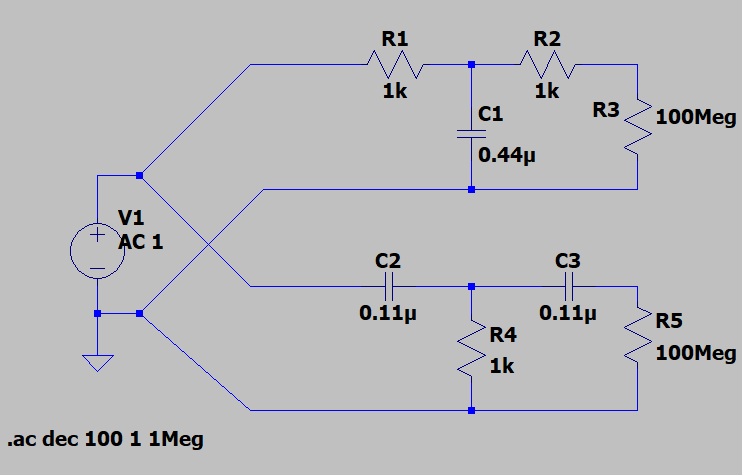
\includegraphics[scale=0.25]{kairozuac2-3.png}
    \caption{(A)の周波数解析での回路図}
\end{figure}
\subsection{結果}
以下にそれぞれの端子の解析結果を示す。ただし、実線は振幅、点線は位相を表す。
\begin{figure}[H]
    \centering
    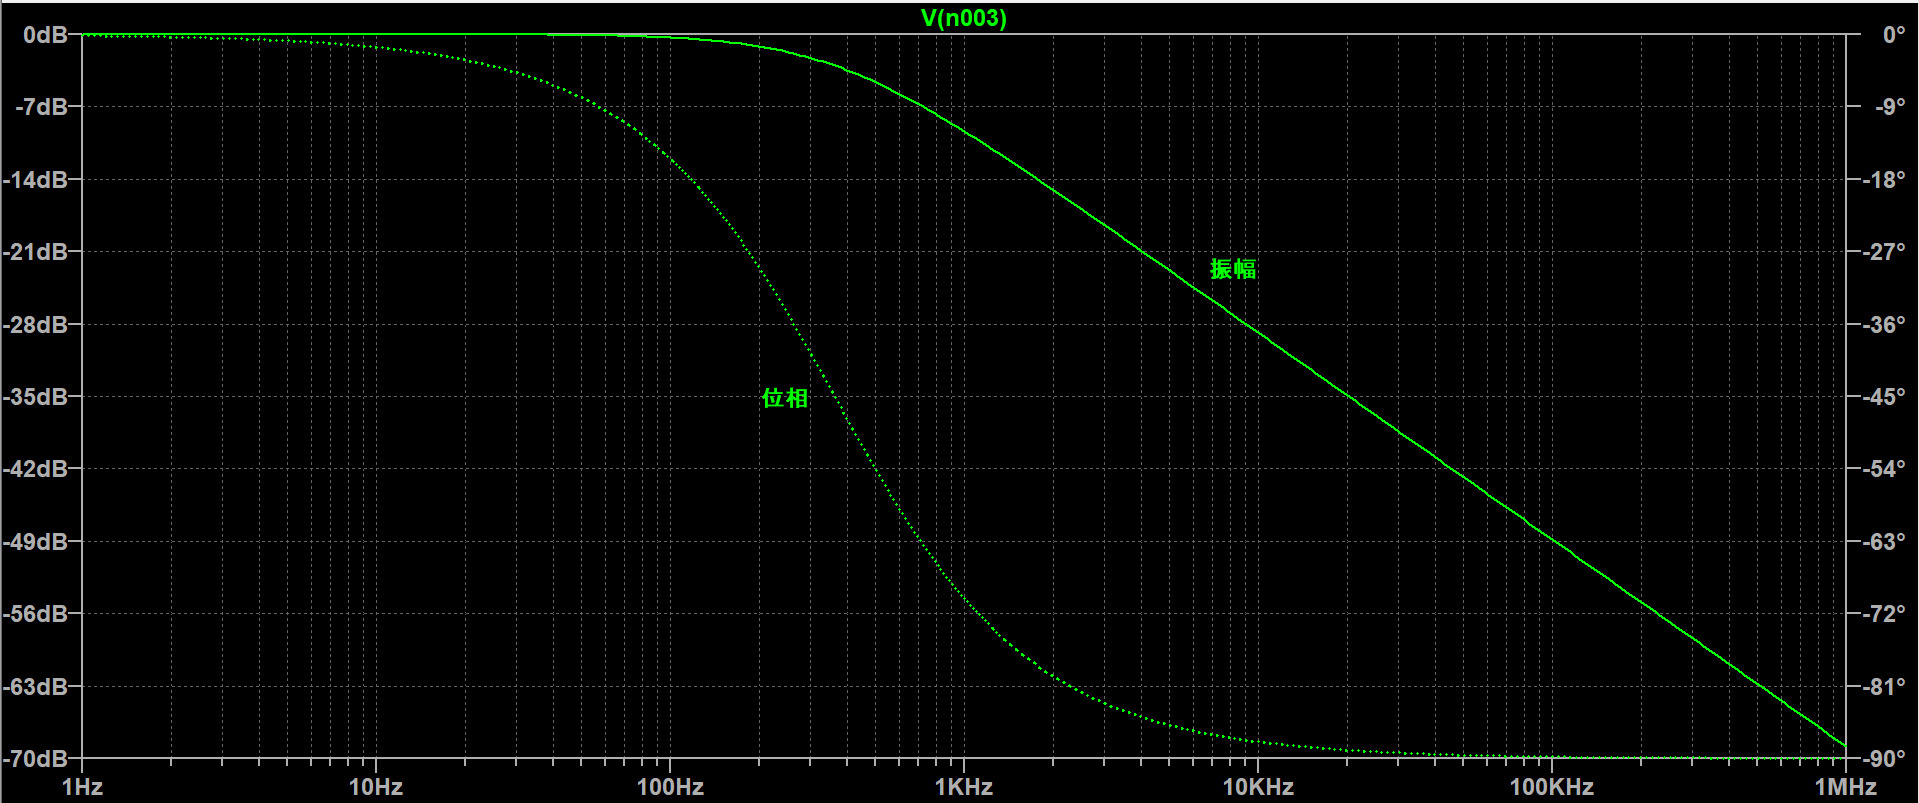
\includegraphics[scale=0.25]{ac1-1.png}
    \caption{端子1-1'}
\end{figure}
\begin{figure}[H]
    \centering
    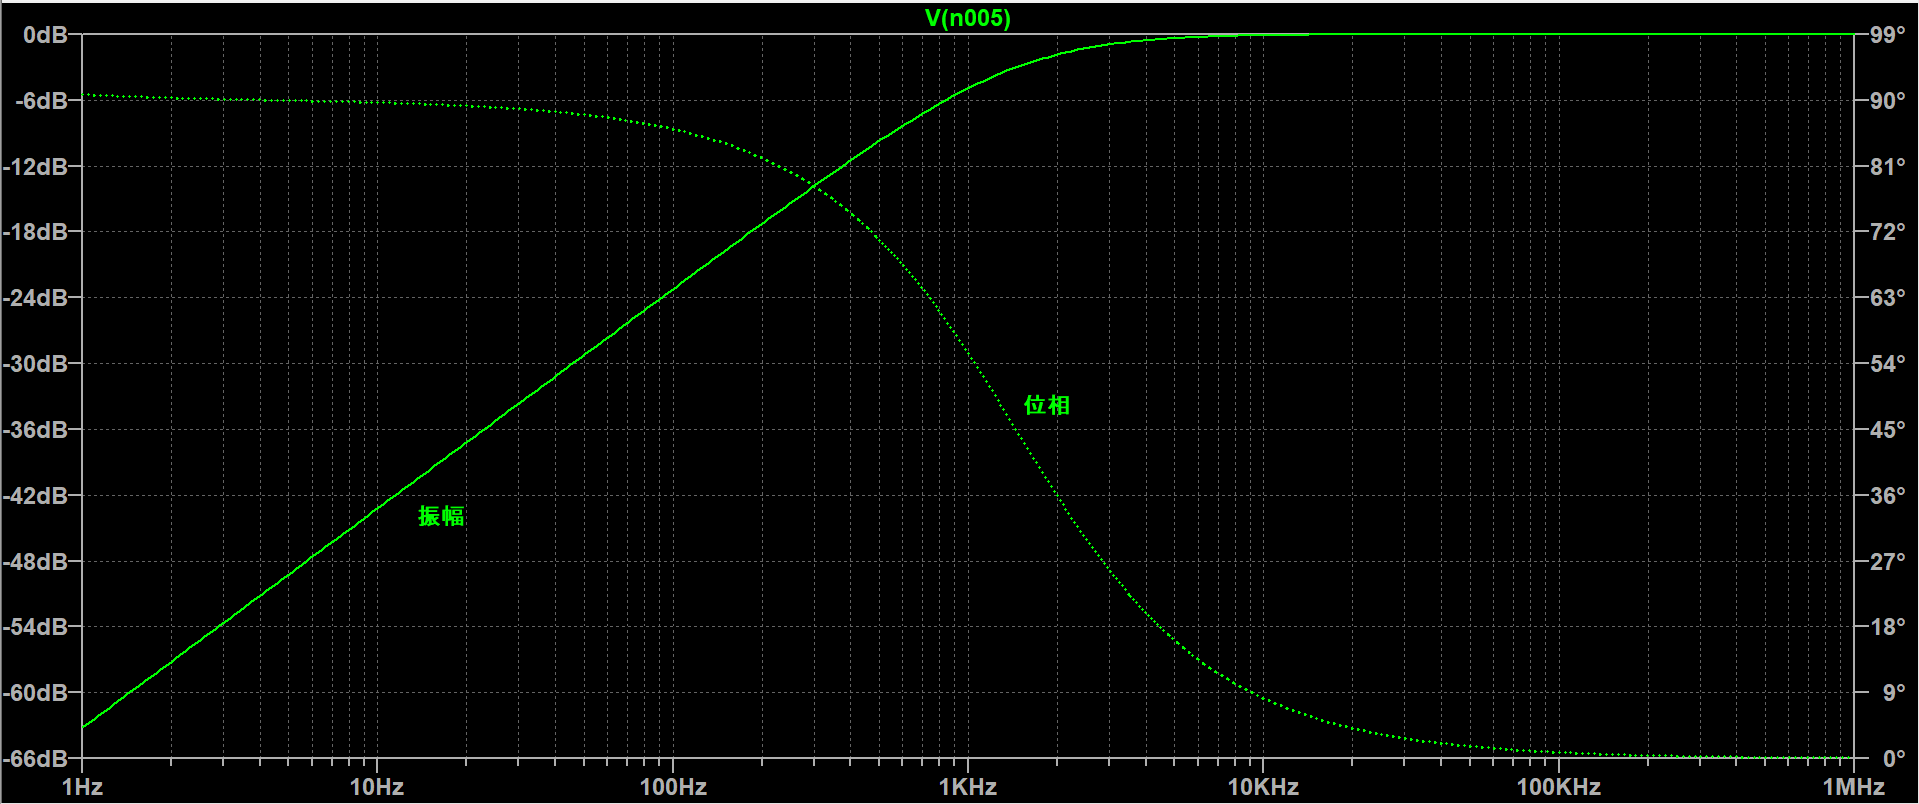
\includegraphics[scale=0.25]{ac2-2.png}
    \caption{端子2-2'}
\end{figure}

\subsection{考察}
振幅特性はデシベル表示を用いて表される。
一般に電力比は
\[
10\log_{10}\left(\frac{P_2}{P_1}\right)
\]
で定義される。

ここで電力は電圧の2乗に比例するため、
電圧比に対しては
\[
20\log_{10}\left(\frac{V_2}{V_1}\right)
\]
となる。

したがって、伝達関数の絶対値を用いて
\[
20\log_{10}\left|H(j\omega)\right|
\]
を振幅特性とした。ここにそれぞれの端子の伝達関数を代入すると、

\begin{align}
20\log_{10}\left|H_1(j\omega)\right|
= 20\log_{10}\frac{1}{\sqrt{1+(2\omega Cr)^{2}}} \notag \\
= 20\log_{10}\frac{1}{\sqrt{1+(4\pi fCr)^{2}}}
\end{align}

\begin{align}
20\log_{10}\left|H_2(j\omega)\right|
&= 20\log_{10}\frac{\omega Cr}{\sqrt{4+(\omega Cr)^{2}}} \notag \\
&= 20\log_{10}\frac{2\pi fCr}{\sqrt{4+(2\pi fCr)^{2}}} \notag \\
&= 20\log_{10}\frac{\pi fCr}{\sqrt{1+(\pi fCr)^{2}}}
\end{align}

位相特性はそれぞれ
\[
-\tan^{-1}(4\pi fCr)
\]
\[
\frac{\pi}{2}-\tan^{-1}(\pi fCr)
\]

以上の結果を用いて、それぞれの振幅特性と位相特性を表にまとめた。
\begin{table}[H]
\centering
\caption{端子1-1'の振幅特性}
\begin{tabular}{ccc}
\hline
$f$ [Hz] & 理論値 [dB] & 測定値 [dB] \\
\hline
1       & -0.0000331931 & -0.000206908 \\
5       & -0.000829751  & -0.00100353 \\
10      & -0.00331805   & -0.00349170 \\
50      & -0.0822002    & -0.0823799 \\
100     & -0.319859     & -0.320026 \\
500     & -4.64006      & -4.64009 \\
1k      & -9.36666      & -9.36675 \\
5k      & -22.8347      & -22.8344 \\
10k     & -28.8383      & -28.8384 \\
50k     & -42.8123      & -42.8119 \\
100k    & -48.8327      & -48.8328 \\
500k    & -62.8121      & -62.8117 \\
1M      & -68.8327      & -68.8327 \\
\hline
\end{tabular}
\end{table}
\begin{table}[H]
\centering
\caption{端子1-1'の位相特性}
\begin{tabular}{ccc}
\hline
$f$ [Hz] & 理論値 [deg] & 測定値 [deg] \\
\hline
1       & -0.158400 & -0.158398 \\
5       & -0.791950 & -0.791942 \\
10      & -1.58360  & -1.58358 \\
50      & -7.87013  & -7.87004 \\
100     & -15.4540  & -15.4539 \\
500     & -54.1168  & -54.1148 \\
1k      & -70.1141  & -70.1140 \\
5k      & -85.8623  & -85.8618 \\
10k     & -87.9284  & -87.9284 \\
50k     & -89.5855  & -89.5855 \\
100k    & -89.7928  & -89.7928 \\
500k    & -89.9586  & -89.9585 \\
1M      & -89.9793  & -89.9793 \\
\hline
\end{tabular}
\end{table}
\begin{table}[H]
\centering
\caption{端子2-2'の振幅特性}
\begin{tabular}{ccc}
\hline
$f$ [Hz] & 理論値 [dB] & 測定値 [dB] \\
\hline
1       & -63.2086   & -63.2095 \\
5       & -49.2292   & -49.2293 \\
10      & -43.2088   & -43.2089 \\
50      & -29.2343   & -29.2344 \\
100     & -23.2292   & -23.2293 \\
500     & -9.71909   & -9.71925 \\
1k      & -4.90438   & -4.90444 \\
5k      & -0.349240  & -0.349305 \\
10k     & -0.0899800 & -0.0899790 \\
50k     & -0.00364000 & -0.00363591 \\
100k    & -0.000910000 & -0.000909081 \\
500k    & -0.0000363662 & -0.0000363741 \\
1M      & -0.00000909157 & -0.00000909175 \\
\hline
\end{tabular}
\end{table}
\begin{table}[H]
\centering
\caption{端子2-2'の位相特性}
\begin{tabular}{ccc}
\hline
$f$ [Hz] & 理論値 [deg] & 測定値 [deg] \\
\hline
1       & 89.9604   & 90.7893 \\
5       & 89.8020   & 89.9678 \\
10      & 89.6040   & 89.6869 \\
50      & 88.0208   & 88.0373 \\
100     & 86.0463   & 86.0546 \\
500     & 70.9361   & 70.9373 \\
1k      & 55.3497   & 55.3508 \\
5k      & 16.1390   & 16.1400 \\
10k     & 8.232780  & 8.232950 \\
50k     & 1.657520  & 1.657640 \\
100k    & 0.828934  & 0.828950 \\
500k    & 0.165798  & 0.165809 \\
1M      & 0.0828991 & 0.0829010 \\
\hline
\end{tabular}
\end{table}
以上の結果より、端子1-1'および端子2-2'の振幅特性および位相特性について、
理論値と測定値は全体としてよく一致していることが確認できた。

まず端子1-1'について、振幅特性は周波数の増加とともに減少しており、
低周波ではほぼ $0\,\mathrm{dB}$ に近く、高周波では大きく減衰している。
また位相特性は周波数の増加に伴って負の方向に変化し、
最終的に $-90^\circ$ に近づいていることが確認できる。

次に端子2-2'については、低周波では振幅が非常に小さく、
周波数の増加とともに振幅が増加し、高周波では $0\,\mathrm{dB}$ に近づいている。
位相特性は低周波では $90^\circ$ 付近の値をとり、
周波数の増加とともに $0^\circ$ に近づいていることが確認できる。

以上より、端子1-1'と端子2-2'では周波数に対する応答が互いに異なっており、
一方が減衰する領域において他方は増加するという関係にあることが分かる。

また、全ての周波数において理論値と測定値は非常によく一致しており、
わずかな差はLTspiceにおける数値計算や読み取り誤差によるものであると考えられる。


\section{実験4}
\subsection{実験内容}
図(B)について周波数解析を行い、
振幅特性および位相特性を求めた。
以下にLTspiceにより作成した回路図を示す。
\begin{figure}[H]
    \centering
    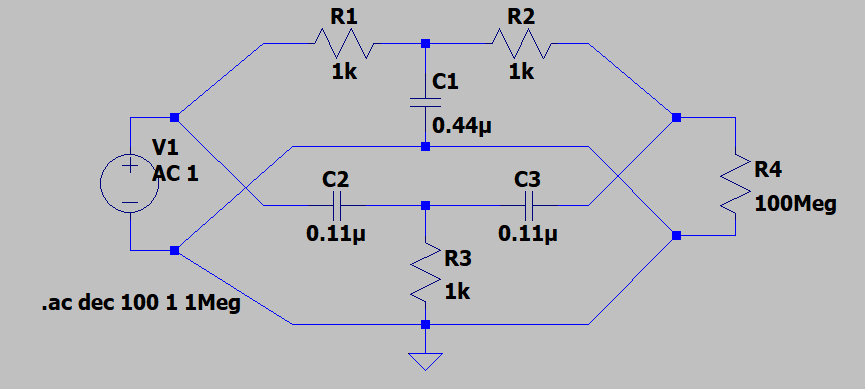
\includegraphics[scale=0.25]{kairozuac2-4.png}
    \caption{(B)の周波数解析での回路図}
\end{figure}

\subsection{結果}
以下に端子3-3'の解析結果を示す。ただし、実線は振幅、点線は位相を表す。
\begin{figure}[H]
    \centering
    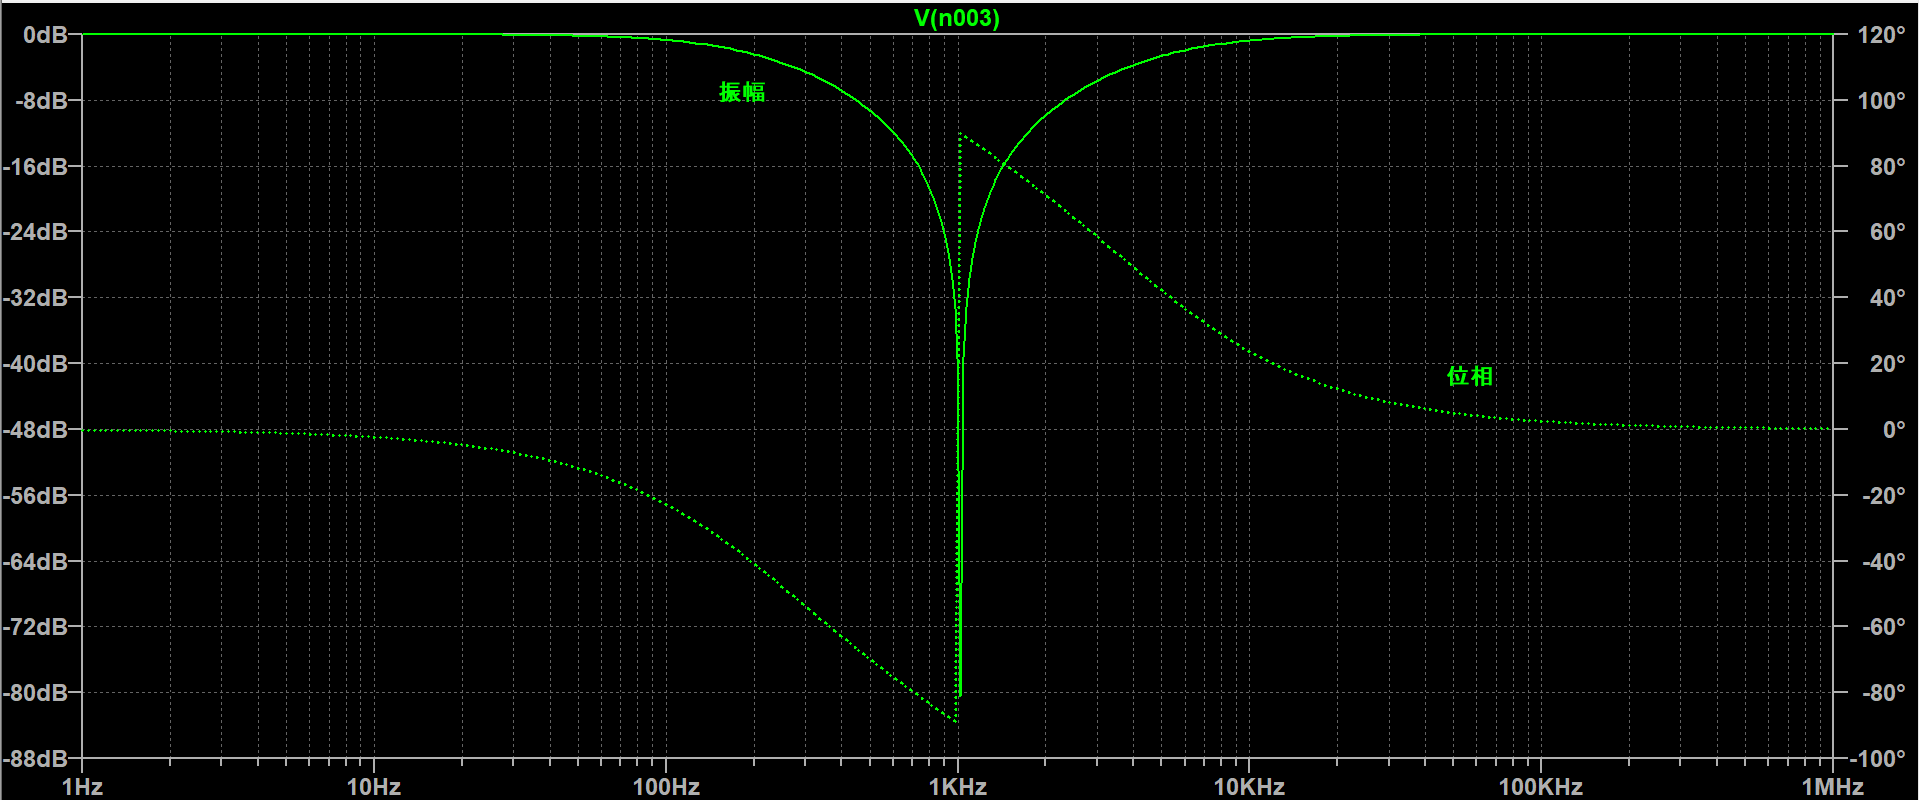
\includegraphics[scale=0.25]{ac2-4.png}
    \caption{端子3-3'}
\end{figure}



\subsection{考察}
実験3と同様にして、振幅特性を求めると
\begin{equation}
20\log_{10}\left|H_B(j\omega)\right|
= 20\log_{10}\left(\frac{\sqrt{(m^6-3m^4+4)^{2}+36(m^5-m^3-2m)^{2}}}
{m^6+33m^4+36m^2+4}\right)
\end{equation}
となる。$m = \omega Cr = 2\pi fCr $となることに注意して、式(36)と式(32)から
各周波数に対する振幅特性と位相特性を求めた。以下にその理論値と測定値をまとめた表を示す。
  \begin{table}[H]
\centering
\caption{端子3-3'の振幅特性}
\begin{tabular}{ccc}
\hline
$f$ [Hz] & 理論値 [dB] & 測定値 [dB] \\
\hline
1       & -0.0000746842 & -0.000248398 \\
5       & -0.00186681   & -0.00204066 \\
10      & -0.00746349   & -0.00763702 \\
50      & -0.183666     & -0.183854 \\
100     & -0.701493     & -0.701651 \\
500     & -9.25345      & -9.25327 \\
1k      & -39.3639      & -39.3640 \\
5k      & -2.60294      & -2.60322 \\
10k     & -0.764270     & -0.764279 \\
50k     & -0.0326342    & -0.0326410 \\
100k    & -0.00817643   & -0.00817652 \\
500k    & -0.000327287  & -0.000327356 \\
1M      & -0.0000818236 & -0.0000818245 \\
\hline
\end{tabular}
\end{table}
\begin{table}[H]
\centering
\caption{端子3-3'の位相特性}
\begin{tabular}{ccc}
\hline
$f$ [Hz] & 理論値 [deg] & 測定値 [deg] \\
\hline
1       & -0.237600 & -0.237596 \\
5       & -1.187860 & -1.187842 \\
10      & -2.374870 & -2.374834 \\
50      & -11.7413  & -11.7411 \\
100     & -22.7186  & -22.7183 \\
500     & -69.8420  & -69.8386 \\
1k      & -89.3835  & -89.3832 \\
5k      & 42.1782   & 42.1787 \\
10k     & 23.6847   & 23.6848 \\
50k     & 4.96358   & 4.96385 \\
100k    & 2.48567   & 2.48569 \\
500k    & 0.497384  & 0.497412 \\
1M      & 0.248696  & 0.248698 \\
\hline
\end{tabular}
\end{table}
以上の結果より、端子3-3'の振幅特性および位相特性について、
理論値と測定値は全体としてよく一致していることが確認できた。

振幅特性については、低周波領域および高周波領域では
$0\,\mathrm{dB}$ に近い値をとり、
中間の周波数帯において大きく減衰していることが分かる。
特に $1\,\mathrm{kHz}$ 付近では振幅が大きく低下しており、
この回路が特定の周波数において出力を抑制する特性を持つことが確認できる。

位相特性については、低周波領域では位相はほぼ $0^\circ$ に近く、
周波数の増加とともに負の方向へ変化し、
$1\,\mathrm{kHz}$ 付近で $-90^\circ$ 近傍となる。
その後、高周波側では再び $0^\circ$ に近づく挙動が確認できる。

また、$1\,\mathrm{Hz}$ においては理論値と測定値にわずかな差が見られるが、
いずれも $0\,\mathrm{dB}$ に極めて近い値であり、
絶対的な差は非常に小さい。
したがって、この差はLTspiceにおける数値計算や読み取り誤差によるものと考えられる。



\section{実験5}
\subsection{実験内容}
図(B)について、ノッチ周波数が
$
9\,\mathrm{kHz}
$
となるようにキャパシタンス $C$ の値を理論式より求めた。

求めた値を回路に適用して再度交流解析を行い、
振幅特性および位相特性を観測し、
ノッチ周波数が所望の値となることを確認した。

\subsection{結果}
ノッチ周波数では振幅特性が0となるため、
伝達関数の分子が0となればよい。

すなわち分子の実部と虚部がともに0となるので、
\[
m^6-3m^4+4=0
\]

\[
6(m^5-m^3-2m)=0
\]
を満たす。

虚部の条件より，
\[
m^5-m^3-2m=0
\]

\[
m(m^4-m^2-2)=0
\]

となる。ここで $m\neq0$ であるから、
\[
m^4-m^2-2=0s
\]
\[
(m^2-2)(m^2+1)=0
\]

より、
\[
m^2=2
\]

したがって、
\[
m=\sqrt{2}
\]

となる。

この値を実部の条件に代入すると、
\[
m^6-3m^4+4
=
(\sqrt{2})^6-3(\sqrt{2})^4+4
\]

\[
=
8-12+4
=
0
\]

となり、実部も0となる。

したがってノッチ条件は
\[
m=\omega Cr=\sqrt{2}
\]

である。

また、
$
\omega=2\pi f
$

より、
\[
2\pi f Cr=\sqrt{2}
\]

したがって、ノッチ周波数は
\[
f_0=
\frac{\sqrt{2}}{2\pi Cr}
\]
で与えられる。

ノッチ周波数を
$f_0=9\,\mathrm{kHz}$
とすると、
\[
C=
\frac{\sqrt{2}}{2\pi r f_0}
\]

である。ここに
$r=1\,\mathrm{k}$
を代入すると、
\[
C=
\frac{\sqrt{2}}{2\pi \times 1000 \times 9000} \\
=25.0\,\mathrm{nF}
\]
となる。

この値を図(B)に入れ、作成した回路図と解析結果を以下に示す。
ただし、実線は振幅、点線は位相を表す。
\begin{figure}[H]
    \centering
    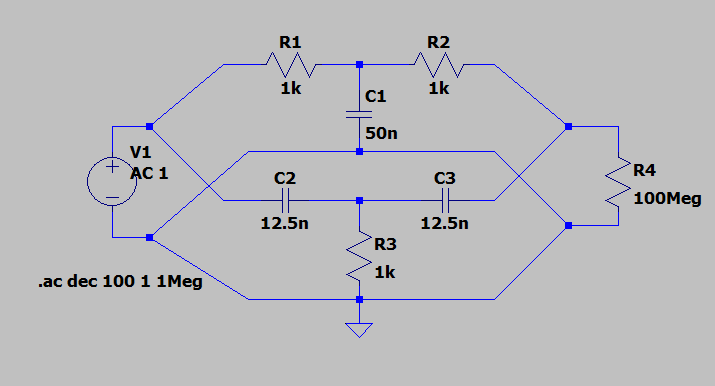
\includegraphics[scale=0.25]{kairozu2-5.png}
    \caption{(B)の変更後の回路図}
\end{figure}
\begin{figure}[H]
    \centering
    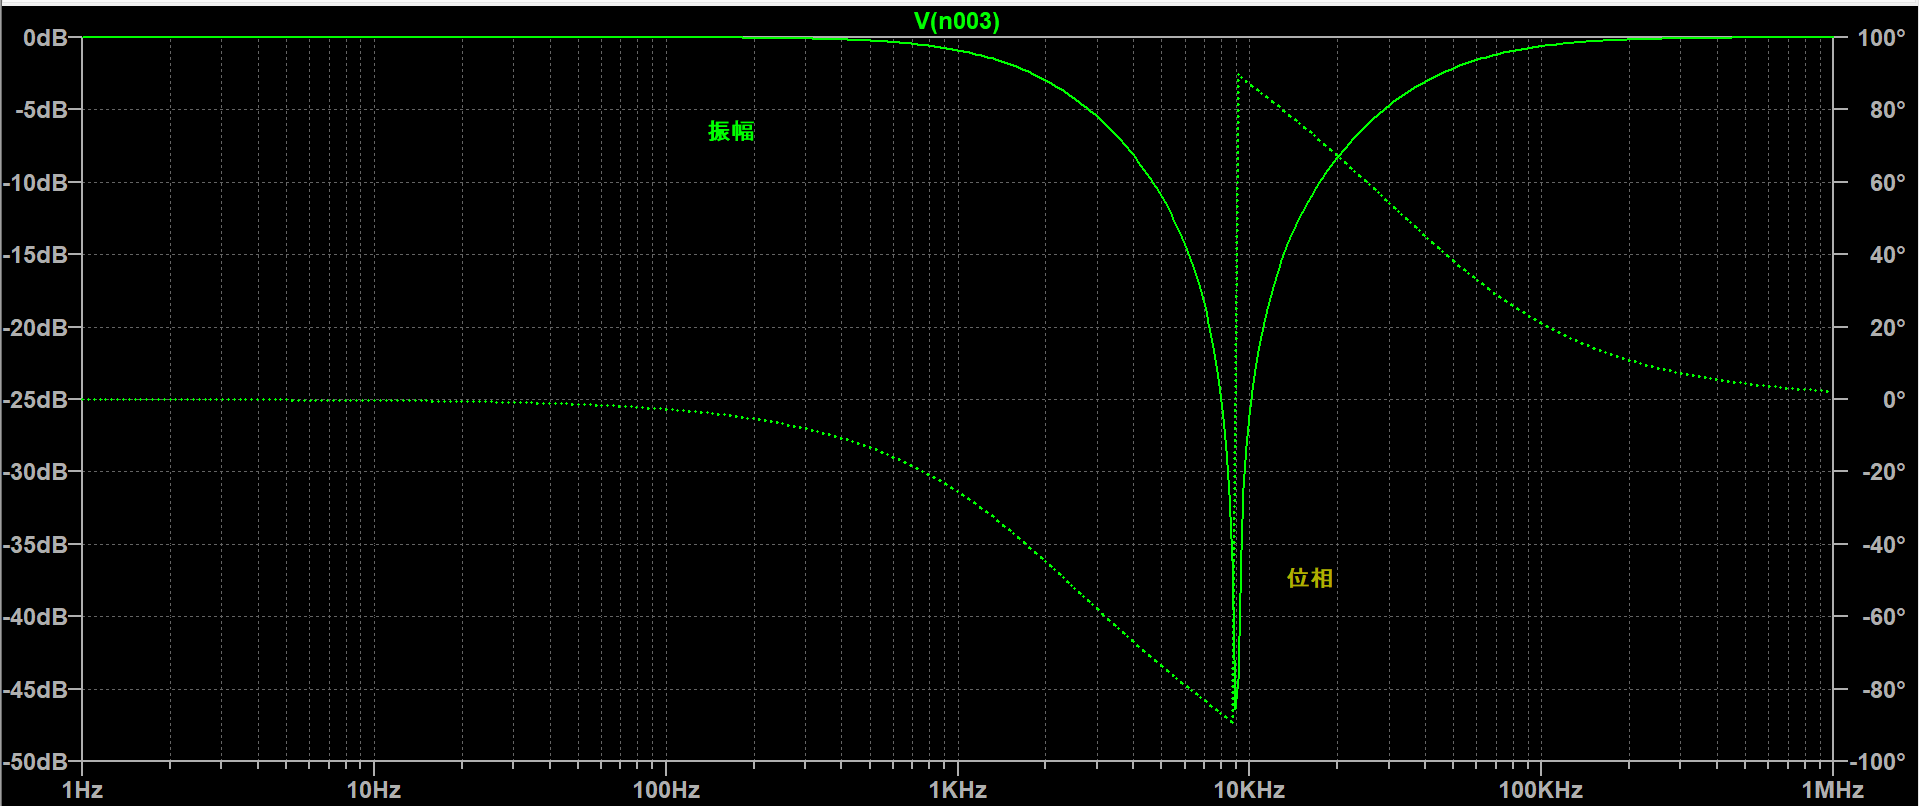
\includegraphics[scale=0.25]{ac2-5.png}
    \caption{(B)の周波数解析(変更後)}
\end{figure}


\subsection{考察}
$m=\sqrt{2}$として式(36)と式(32)から
各周波数に対する振幅特性と位相特性を求めた。以下にその理論値と測定値をまとめた表を示す。
\begin{table}[H]
\centering
\caption{端子3-3'の振幅特性}
\begin{tabular}{ccc}
\hline
$f$ [Hz] & 理論値 [dB] & 測定値 [dB] \\
\hline
1       & -0.000000964421 & -0.000174680 \\
5       & -0.0000241105   & -0.000197828 \\
10      & -0.0000964412   & -0.000270155 \\
50      & -0.00241053     & -0.00258442 \\
100     & -0.00963589     & -0.00980937 \\
500     & -0.236066       & -0.236254 \\
1k      & -0.890740       & -0.890894 \\
5k      & -11.0063        & -11.0061 \\
10k     & -26.1023        & -26.1024 \\
50k     & -2.10420        & -2.10445 \\
100k    & -0.600542       & -0.600548 \\
500k    & -0.0252885      & -0.0252938 \\
1M      & -0.00633287     & -0.00633294 \\
\hline
\end{tabular}
\end{table}

\begin{table}[H]
\centering
\caption{端子3-3'の位相特性}
\begin{tabular}{ccc}
\hline
$f$ [Hz] & 理論値 [deg] & 測定値 [deg] \\
\hline
1       & -0.0270000 & -0.0269996 \\
5       & -0.1349998 & -0.134998 \\
10      & -0.2699983 & -0.269995 \\
50      & -1.34979  & -1.34977 \\
100     & -2.69834  & -2.69830 \\
500     & -13.2977  & -13.2975 \\
1k      & -25.5070  & -25.5067 \\
5k      & -73.6423  & -73.6386 \\
10k     & 87.1609   & 87.1611 \\
50k     & 38.2926   & 38.2932 \\
100k    & 21.0614   & 21.0615 \\
500k    & 4.37000   & 4.37024 \\
1M      & 2.18765   & 2.18767 \\
\hline
\end{tabular}
\end{table}

振幅特性について理論値と測定値を比較すると，全体としてよく一致しており、
特にノッチ付近では大きな減衰が得られ、
回路が特定の周波数成分を強く抑制する性質を持つことが明確に示された。

一方で、低周波および高周波領域では振幅は $0\,\mathrm{dB}$ に近づいており、
ノッチ周波数以外の成分はほとんど減衰しないことが分かる。
位相特性についても理論値と測定値はほぼ一致しており、
周波数による位相変化が理論通りに再現されていることが確認できた。
\section{感想}
今回の実験では特にノッチ周波数を扱う実験が印象的だった。
キャパシタの値を変えることで特定の周波数を大きく減衰させられるという性質は興味深い。
ノッチ特性の利用場面について調べると，音響機器におけるハウリングの抑制や，通信システムなど，
様々な場面で利用されていることが分かった。
このことから，ノッチ特性は非常に実用性の高い特性であることが分かった。
\begin{thebibliography}{99}
    \bibitem{tex}
    【ノッチフィルタとは】設計方法や用途について　\url{https://detail-infomation.com/notch-filter/}
    ノッチ フィルター設計:特定のノイズ減衰のための狭帯域フィルター　\url{https://ja.mfgrobots.com/mfg/it/1007029669.html#google_vignette}

\end{thebibliography}




















\end{document}